\chapter{試作したツールの実装}\label{cha:Implementation}
本研究では、帳票のレイアウトを変更せず、電子フォーム作成にかかる手間と時間を削減することを目的として、記入欄自動検出およびラベル割付ツールを試作する。
試作するツールは、領域座標取得部、文字情報取得部、ラベル割付部、ファイル出力部の4つの処理部で構成する。
試作するツールの構成を、図\ref{fig:structure}に示す。

\begin{figure}[tp]
    \begin{center}
        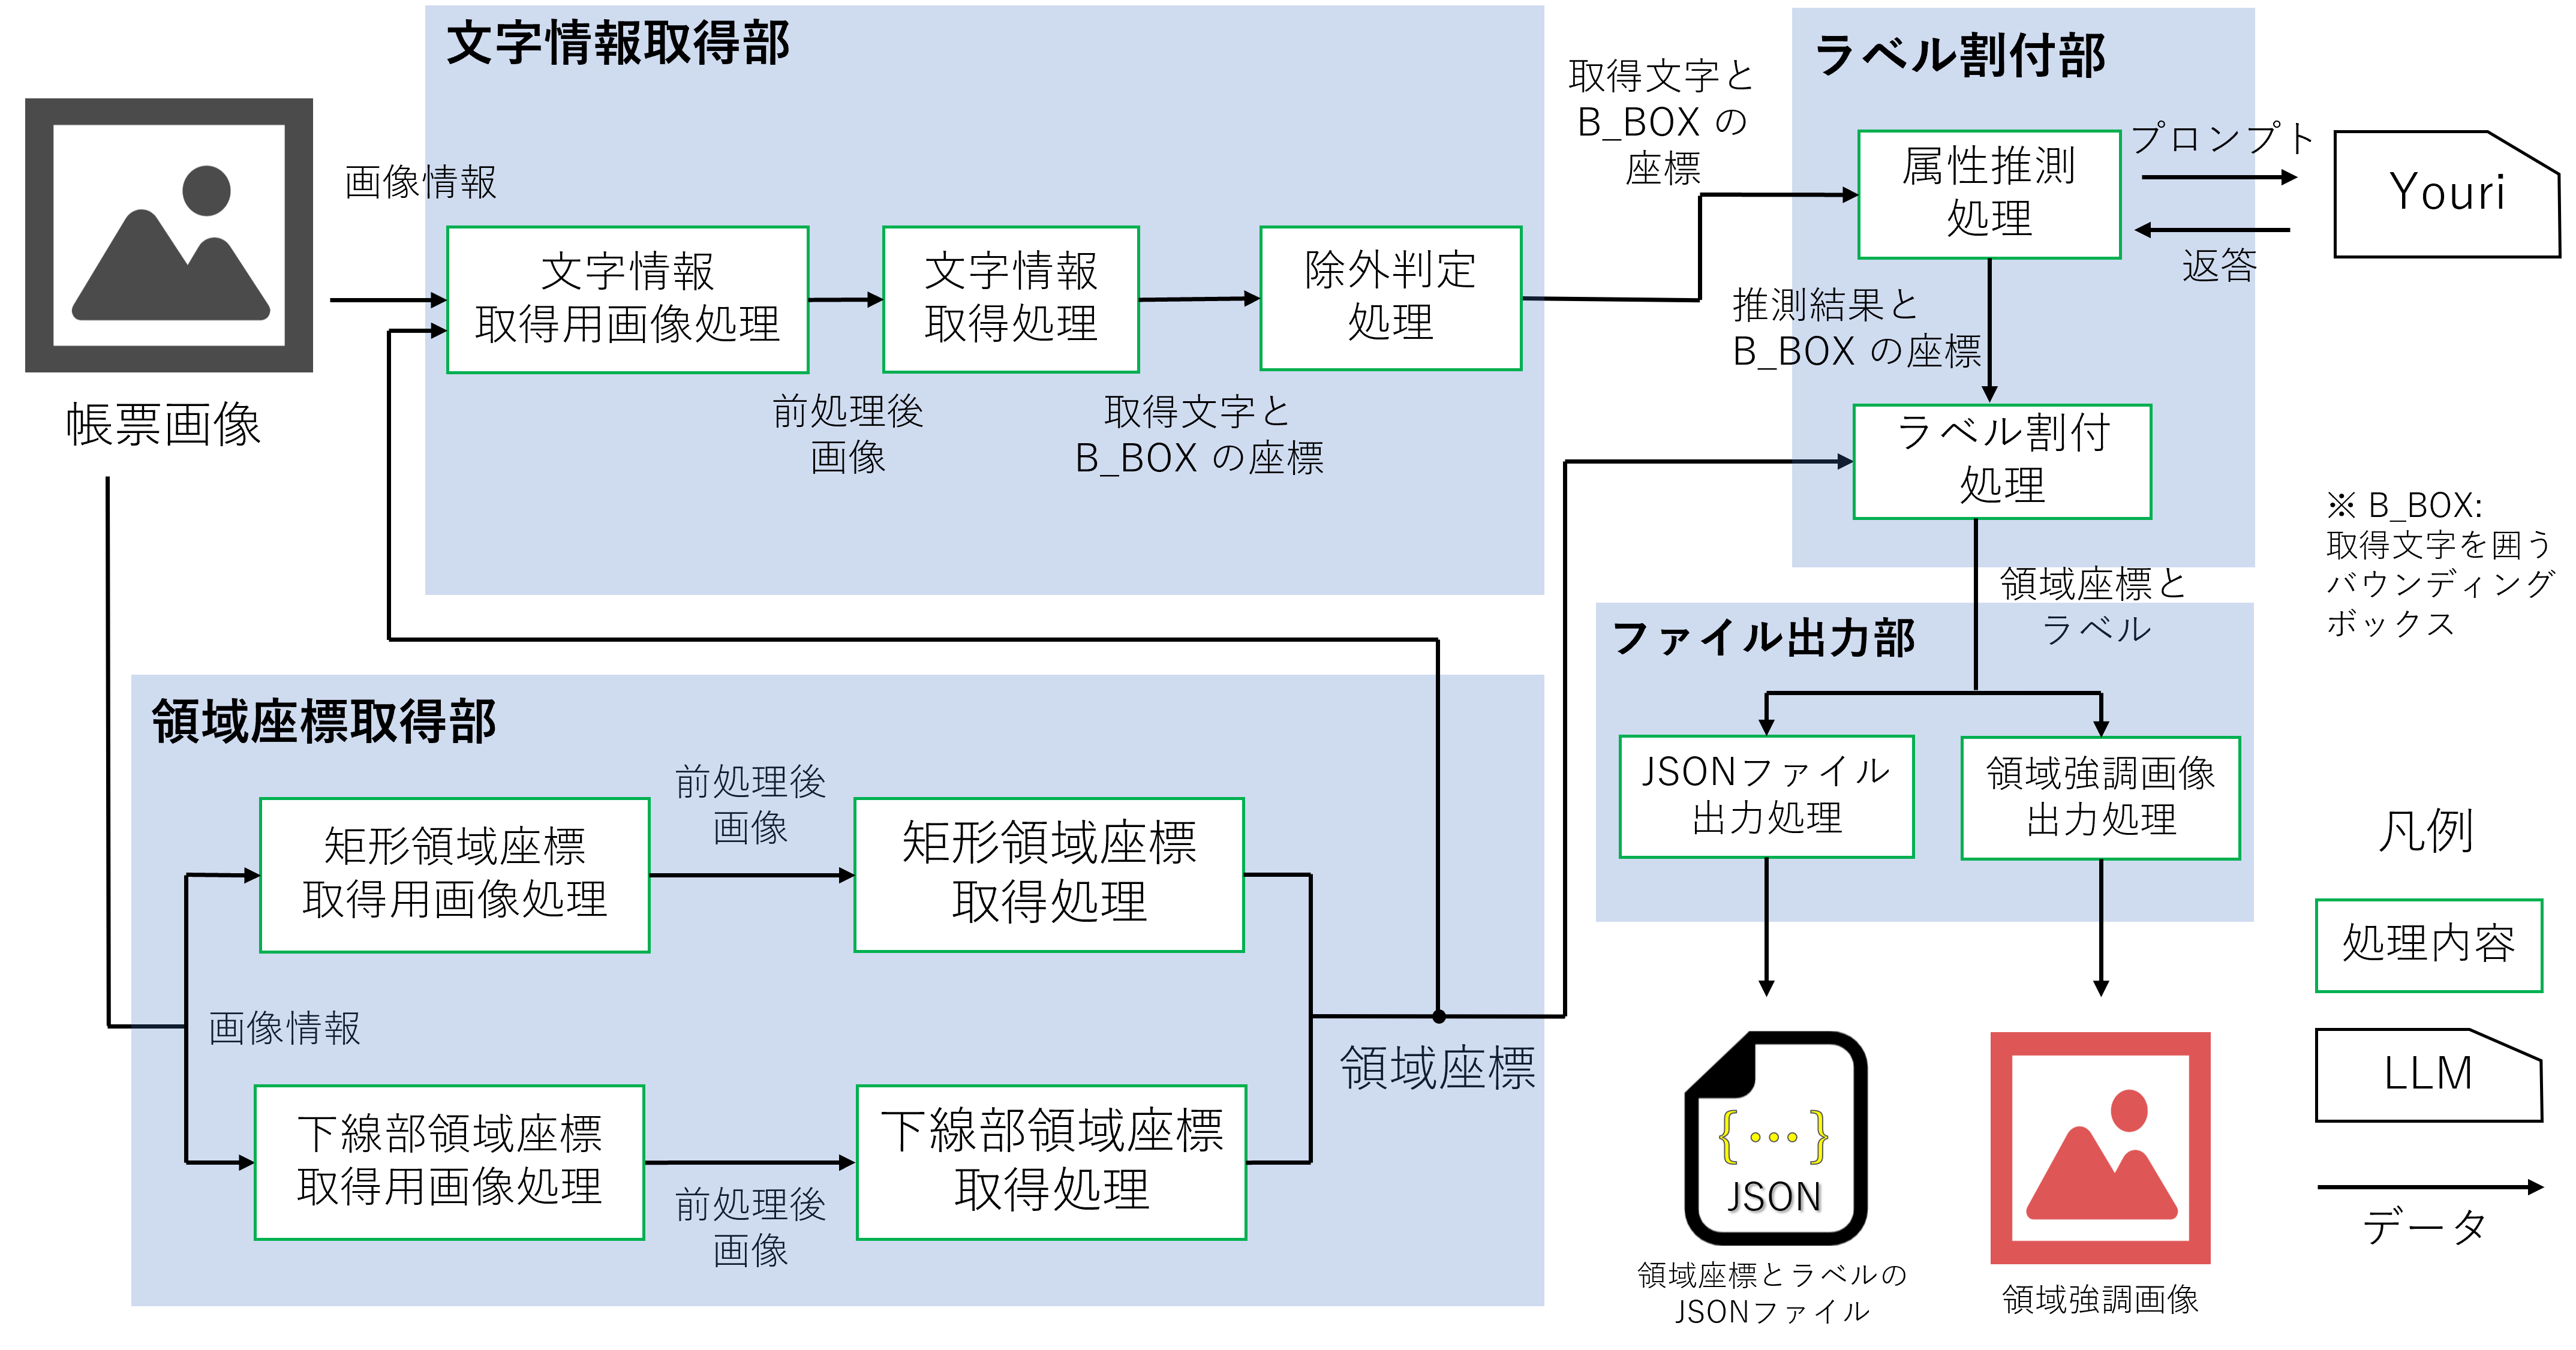
\includegraphics[width=15cm]{image/04-implementation/structure.png}
        \caption{試作するツールの構造}
        \label{fig:structure}
    \end{center}
\end{figure}

以降、本章では4つの処理部について説明する。


\section{領域座標取得部}\label{sec:area_coords_obtainment_part}
領域座標取得部は、帳票画像内記入欄を検出し、領域座標を取得する処理部である。
帳票画像を入力とし、領域座標を出力とする。
出力は、文字情報取得部(\ref{sec:OCR_part}節で後述)とラベル割付部(\ref{sec:label_link_part}節で後述)に渡す。

矩形の帳票画像内記入欄については各頂点の4つのxy座標を、下線部の帳票画像内記入欄については両端点の2つのxy座標を、それぞれ領域座標として取得する。

% 矩形
\subsection{矩形領域座標取得用画像処理}\label{subsec:image_processing_for_rect_coords_obtainment}
矩形領域座標取得用画像処理は、矩形領域の検出精度を高めるため、複数の画像処理を行う処理である。
帳票画像を入力とし、膨張処理後の二値画像を出力とする。
出力は、矩形領域座標取得処理(\ref{subsec:rect_coords_obtainment_processing}節で後述)に渡す。

試作するツールでは、矩形の取得にあたり、OpenCVのfindContours関数(\ref{sec:OpenCV}節を参照)を用いる。
この関数を呼び出すとき、第一引数に渡すパスが示す処理画像の画素に、白色と黒色以外の画素が存在する場合、エラーが発生してしまうため、処理画像を二値化する必要がある。
また、矩形の検出精度を高めるため、後述する画像処理を組み合わせ、二値化する。

本処理で行う画像処理の流れを、以下に示す。

\begin{enumerate}
    \item 画像の読み込み\\
        OpenCVのimread関数(\ref{sec:OpenCV}節を参照)を用いて、帳票画像を読み込む。
        帳票画像のパスを入力として、読み込んだ帳票画像の多次元配列を出力し、cvtColor関数(\ref{sec:OpenCV}節を参照)に渡す。
    \item 帳票画像のグレースケール化\\
        OpenCVのcvtColor関数を用いて、画像をグレースケール化することにより、色情報を削減し、計算量を減らすことで処理を高速化する。
        imread関数で読み込んだ帳票画像を受け取り、グレースケール化した帳票画像を出力し、DeblulrGANv2(\ref{sec:DeblurGANv2}節を参照)に渡す。
        以降、グレースケール化した帳票画像を、グレースケール帳票画像と呼ぶ。
    \item ブレ除去後のグレースケール化帳票画像の生成\\
        DeblurGANv2を適用することにより、帳票画像を撮影する際に発生する画像内のブレを除去し、矩形の検出精度を高める。
        グレースケール帳票画像を受け取り、ブレ除去後のグレースケール帳票画像を出力し、GaussianBlur関数(\ref{sec:OpenCV}節を参照)に渡す。
    \item ノイズ除去\\
        OpenCVのGaussianBlur関数を用いて、画像内のノイズを除去し、ノイズを矩形として検出することを防ぐ。
        なお、3行3列の矩形カーネルを使用し、標準偏差を0とする。
        ブレ除去後のグレースケール帳票画像を受け取り、ブレ除去およびノイズ除去後のグレースケール化帳票画像を出力し、threshold関数(\ref{sec:OpenCV}節を参照)に渡す。
    \item 二値画像への変換\\
        OpenCVのthreshold関数を用いて、大津の二値化による閾値処理を行う。
        閾値の決定手法を指定する変数は、THRESH\_TOZERO\_INVに指定して二値化する。
        これは、findContours関数(\ref{sec:OpenCV}節を参照)が黒い背景にある白い領域の輪郭を検出するためである。
        ブレ除去およびノイズ除去後のグレースケール化帳票画像を受け取り、二値化した帳票画像を出力し、dilate関数(\ref{sec:OpenCV}節を参照)に渡す。
    \item カーネルの作成\\
        getStructuringElement関数(\ref{sec:OpenCV}節を参照)を用いて、5行5列の矩形カーネルを作成する。
        カーネルの形状を決定する第一引数の変数については、MORPH\_RECTを用いる。
        設定する引数を受け取り、カーネルを出力し、dilate関数に渡す。
    \item 膨張処理\\
        getStructuringElement関数で作成した矩形カーネルを用いる。
        OpenCVのdilate関数(\ref{sec:OpenCV}節を参照)を用いて、膨張処理で矩形の辺を太くすることで、検出精度を高める。
        なお、膨張する回数は1回とする。
        カーネルと二値化した帳票画像を受け取り、膨張処理後の二値化した帳票画像を出力し、矩形領域座標取得処理に渡す。
\end{enumerate}

なお、下線部領域座標取得用画像処理(\ref{subsec:image_processing_for_underline_coords_obtainment}節で後述)で行うエッジ検出は、矩形領域座標取得用画像処理では行わない。
これは、矩形の辺を境界として、内側と外側に矩形を認識してしまい、不要に矩形領域を取得することを防ぐためである。

\subsection{矩形領域座標取得処理}\label{subsec:rect_coords_obtainment_processing}
矩形領域座標取得処理は、膨張処理後の二値化した帳票画像を入力として、矩形の帳票画像内記入欄を検出し、矩形領域座標を取得する処理である。
矩形領域座標取得用画像処理(\ref{subsec:image_processing_for_rect_coords_obtainment})の膨張処理後の二値画像を入力として、矩形領域座標を出力とする。
出力は、下線部領域座標取得処理(\ref{subsec:underline_coords_obtainment_processing}節で後述)、文字情報取得用画像処理(\ref{subsec:image_processing_for_char_recognition}節で後述)、ラベル割付処理(\ref{subsec:label_link_processing}節で後述)へ渡す。

膨張処理後の二値化した帳票画像に対して、OpenCVのfindContours関数(\ref{sec:OpenCV}節を参照)による輪郭検出を用いて、矩形の帳票画像内記入欄を検出する。
なお、以下の条件のいずれかに該当する矩形については、除去できなかったノイズを矩形として誤検知した可能性が高いとして、出力の対象外とする。

\begin{itemize}
    \item 面積が3000ピクセル以下である場合
    \item 一辺の長さが10ピクセル以下である場合
\end{itemize}

% 下線部
\subsection{下線部領域座標取得用画像処理}\label{subsec:image_processing_for_underline_coords_obtainment}
下線部領域座標取得用画像処理は、下線部領域座標の検出精度を高めるため、複数の画像処理を行う処理である。
帳票画像を入力とし、エッジを強調した二値化後の帳票画像を出力とする。
出力は、下線部領域座標取得処理(\ref{subsec:underline_coords_obtainment_processing}で後述)に渡す。

試作するツールでは、下線部の取得にあたり、OpenCVのHoughLinesP関数(\ref{sec:OpenCV}節を参照)による、ハフ変換を用いた直線検出を行う。
この関数を呼び出すとき、第一引数に渡すパスが示す処理画像の画素に、白色と黒色以外の画素が存在する場合、エラーが発生してしまうため、処理画像を二値化する必要がある。
また、直線の検出精度を高めるため、後述する画像処理を組み合わせ、二値化する。

本処理で行う画像処理の流れを、以下に示す。
なお、本処理における画像処理の一部は、矩形領域座標取得処理(\ref{subsec:rect_coords_obtainment_processing}節を参照)と同様の画像処理を行う。

\begin{enumerate}
    \item 画像の読み込み\\
        OpenCVのimread関数を用いて、帳票画像を読み込む。
        帳票画像のパスを入力として、読み込む帳票画像の配列を出力する。
        出力する帳票画像の配列は、cvtColor関数に渡す。
    \item 帳票画像のグレースケール化\\
        OpenCVのcvtColor関数を用いて、画像をグレースケール化することにより、色情報を削減し、計算量を減らすことで処理を高速化する。
        帳票画像の配列を受け取り、グレースケール化帳票画像の配列を出力する。
        出力する帳票画像の配列は、DeblurGANv2に渡す。
    \item ブレ除去後のグレースケール化帳票画像の生成\\
        DeblurGANv2を適用することにより、帳票画像を撮影する際に発生する画像内のブレを除去し、下線部の検出精度を高める。
        グレースケール化帳票画像の配列を受け取り、ブレ除去後のグレースケール化帳票画像の配列を出力する。
        出力する帳票画像の配列は、threshold関数に渡す。
    \item 二値画像への変換\\
        OpenCVのthreshold関数を用いて、大津の二値化による閾値処理を行う。
        閾値の決定手法を指定する変数をTHRESH\_BINARYに指定して二値化する。
        ブレ除去後のグレースケール化帳票画像の配列を受け取り、二値化した帳票画像の配列を出力する。
        出力する帳票画像の配列は、Canny関数(\ref{sec:OpenCV}節を参照)に渡す。
    \item エッジ検出\\
        Canny関数を用いて、エッジ検出を行う。
        閾値処理における上限と下限の閾値を、以下のように決定する。
        \begin{enumerate}
            \item 大津の二値化で取得した閾値を受け取る。
            \item 二値画像を対象に、画素値の中央値を定数倍(本研究では定数を0.33とする)し、取得した閾値から加減算する。
            \item 加算した値を上限の閾値、減算した値を下限の閾値として、それぞれ設定する。
        \end{enumerate}
        二値化した帳票画像を受け取り、エッジを強調した二値化後の帳票画像の配列を出力する。
        出力する帳票画像の配列は、下線部領域座標取得処理に渡す。
\end{enumerate}

なお、矩形領域座標取得用画像処理(\ref{subsec:image_processing_for_rect_coords_obtainment}節を参照)で行った膨張処理は、下線部領域座標取得用画像処理では行わない。
これは、膨張処理によって黒色と白色の境界がぼやけてしまい、エッジ検出が失敗し、下線部の検出精度が低下することを防ぐためである。

\subsection{下線部領域座標取得処理}\label{subsec:underline_coords_obtainment_processing}
下線部領域座標取得処理は、下線部の帳票画像内記入欄を検出し、下線部領域座標を取得する処理である。
下線部領域座標取得用画像処理(\ref{subsec:image_processing_for_underline_coords_obtainment}節を参照)のエッジを強調した二値化後の帳票画像と、矩形領域座標取得処理(\ref{subsec:rect_coords_obtainment_processing}節を参照)の矩形領域座標を入力とし、下線部領域座標を出力とする。
出力は、文字情報取得用画像処理(\ref{subsec:image_processing_for_char_recognition}節で後述)とファイル出力部(\ref{subsec:file_output_part}節で後述)へ渡す。

画像処理後、OpenCVのHoughLinesP関数によるハフ変換を用いて、下線部の帳票画像内記入欄を検出する。
なお、以下の条件のいずれかに該当する直線については、誤検出の可能性が高いとして、出力の対象外とする。
矩形領域座標取得処理(\ref{subsec:rect_coords_obtainment_processing}節を参照)の出力を、判定する条件の1つに用いる。

\begin{itemize}
    \item 直線の長さが10ピクセル未満である場合\\
        Canny法によるエッジ検出の際に適用するガウシアンフィルタで、除去できていないノイズによって誤検出したエッジを下線部と捉えることを防ぐ。
    \item 水平を基準として傾きが3ピクセル以上である場合\\
        横書きの帳票において、下線部の直線は水平であるため、垂直な直線を下線部と捉えることを防ぐ。
    \item 直線が矩形領域の辺の一部から上下20ピクセル以内に存在する場合\\
        矩形領域座標取得処理の出力を判定に利用する。矩形領域の辺の一部を下線部と捉えることを防ぐ。
\end{itemize}

HoughLinesP関数によって直線を検出する際、入力画像内にある1本の直線の上下に、誤って2本の直線を検出してしまう不具合が発生する場合がある。
これは、両端点のxy座標が1ピクセル単位で異なる直線を、別の直線として検出するためである。
この不具合の発生を防ぐため、検出した直線の中点を全て計算し、ある直線における中点のy座標について、上下10ピクセル以内に別の直線の中点が存在する場合は、二直線の両端点のxy座標をそれぞれ平均して1本の直線に統一する。

\section{文字情報取得部}\label{sec:OCR_part}
文字情報取得部では、光学文字認識(\ref{sec:Optical-Charactor-Recognition}節を参照)によって、帳票画像内の文字情報を取得する処理部である。
帳票画像を入力とし、文字情報を出力する。
出力は、ラベル割付部(\ref{sec:label_link_part}節で後述)に渡す。

なお、試作するツールでは、光学文字認識ソフトTesseract-OCR\cite{Tesseract-OCR}を用いる。

\subsection{文字情報取得用画像処理}\label{subsec:image_processing_for_char_recognition}
文字情報取得用画像処理は、帳票画像に対して、文字情報を取得するための画像処理を行う処理である。
帳票画像を入力とし、二値化した帳票画像を出力とする。
出力は、下線部領域座標取得処理(\ref{subsec:underline_coords_obtainment_processing}で後述)に渡す。

文字の認識精度を高めるため、帳票画像に対し、複数の画像処理を行う。

本処理で行う画像処理の流れを、以下に示す。

\begin{enumerate}
    \item 画像の読み込み\\
        OpenCVのimread関数を用いて、帳票画像を読み込む。
        帳票画像のパスを入力として、読み込む帳票画像の配列を出力する。
        出力する帳票画像の配列は、drawContours関数とline関数に渡す。
    \item 領域座標の取得\\
        領域座標取得部(\ref{sec:area_coords_obtainment_part}節を参照)から、領域座標を取得する。
        取得する領域座標を、drawContours関数とline関数に渡す。
    \item 背景色のRGB値を取得\\
        背景色は、画像内で占める面積が最も広い色である。
        全画素のRGB値を取得し、最も取得回数が多いRGB値を、背景色のRGB値とする。
        Numpyのhistogram関数(\ref{sec:Numpy}節を参照)を用いて、各色空間の値について、それぞれのヒストグラムを、ビンの数を256として作成し、3つの最頻値のビンを取得する。
        各色空間の値は、それぞれ下限が0、上限が255であるため、1単位で各色空間の最頻値を計算する。
        3つの最頻値を組み合わせ、取得する背景色のRGB値を、drawContours関数とline関数に渡す。
    \item 背景色での矩形領域と下線部領域の描画\\
        OpenCVのdrawContours関数とOpenCVのline関数を用いて、矩形領域と下線部領域を、背景色でそれぞれ描画することによって、文字でない黒色の画素を減らす。
        これにより、文字でない黒色の画素値によって、大津の二値化で計算する閾値が変化することを防ぐ。
        試作するツールでは、太さ15ピクセルの矩形と直線を描画する。
        帳票画像、取得する領域座標、背景色のRGB値を受け取り、背景色で領域を描画した帳票画像の配列を出力する。
        出力する帳票画像の配列は、cvtColor関数に渡す。
    \item 帳票画像のグレースケール化\\
        OpenCVのcvtColor関数を用いて、画像をグレースケール化することにより、色情報を削減し、計算量を減らすことで処理を高速化する。
        背景色で領域を描画した画像を受け取り、背景色で領域を描画したグレースケール化帳票画像の配列を出力する。
        出力する帳票画像の配列は、DeblurGANv2に渡す。   
    \item ブレ除去後の帳票画像の生成\\
        DeblurGANv2を適用することにより、帳票画像を撮影する際に発生する画像内のブレを除去し、光学文字認識の精度を高める。
        背景色で領域を描画したグレースケール化帳票画像を受け取り、ブレ除去後の背景色で領域を描画したグレースケール化帳票画像を出力する。
        出力する帳票画像の配列は、drawContours関数(\ref{sec:OpenCV}節を参照)とline関数(\ref{sec:OpenCV}節を参照)に渡す。
    \item 二値画像への変換\\
        OpenCVのthreshold関数を用いて、大津の二値化による閾値処理を行う。
        閾値の決定手法を指定する変数をTHRESH\_BINARYに指定して二値化する。
        ブレ除去後の背景色で領域を描画したグレースケール化帳票画像を受け取り、二値化した帳票画像を出力する。
        出力する帳票画像の配列は、文字情報取得処理に渡す。
\end{enumerate}

光学文字認識の精度を高めるため、背景色のRGB値を取得し、その色で矩形領域と下線部領域を描画している。
これは、大津の二値化によって決定した閾値が、矩形領域の辺上と下線部領域の直線上の画素値を参照し、光学文字認識の精度が低くなることを防ぐためである。
\ref{sec:input_images}節で述べたように、背景が白色である帳票を対象としているが、白色であることを示す(255,255,255)のRGB値で領域を描画すると、以下のような問題が発生する。

ある電子化文書の帳票画像のうち、矩形領域の一部を、図\ref{fig:before_background_coloring}に示す。
図\ref{fig:before_background_coloring}の元である電子文書の帳票画像は、背景色は完全な白色だった。
しかし、帳票画像を印刷し、カメラで撮影したことによって、印刷用紙の色と撮影する照明の影響により、やや黄色に変化している。
これを防ぐため、背景色のRGB値を取得する必要がある。

図\ref{fig:before_background_coloring}に対して、取得した矩形領域を背景色で描画した帳票画像の一部を、図\ref{fig:after_background_coloring}に示す。
\begin{figure}[tp]
    \centering
    \begin{minipage}[c]{0.45\linewidth}
        \centering
        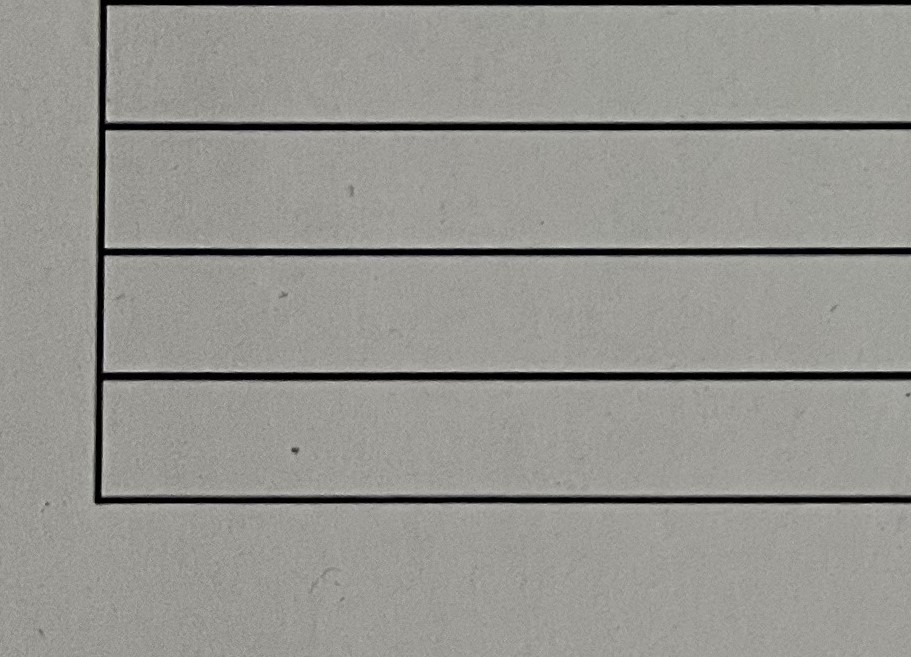
\includegraphics[keepaspectratio, width=7cm]{image/04-implementation/before_background_coloring.jpg}
        \caption{ある電子化文書の帳票画像における矩形領域の一部}
        \label{fig:before_background_coloring}
    \end{minipage}
    \begin{minipage}[c]{0.45\linewidth}
        \centering
        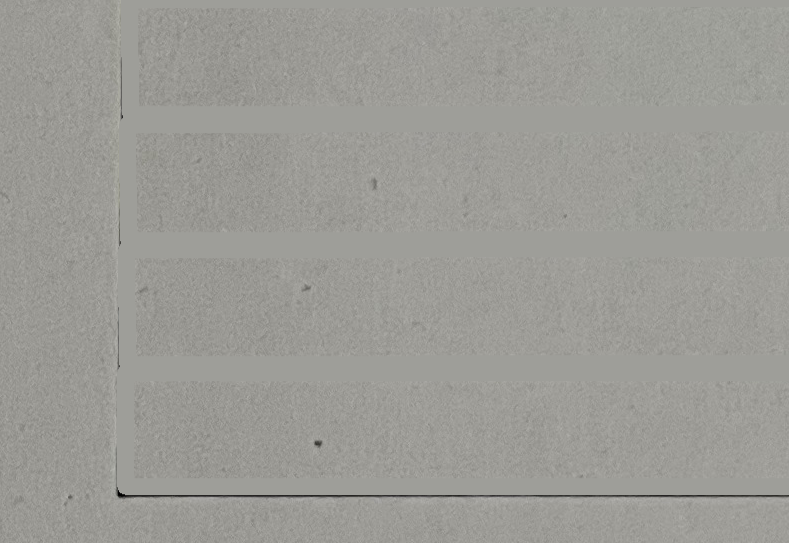
\includegraphics[keepaspectratio, width=7cm]{image/04-implementation/after_background_coloring.png}
        \caption{図\ref{fig:before_background_coloring}の矩形領域を背景色で描画した画像}
        \label{fig:after_background_coloring}
    \end{minipage}
\end{figure}
図\ref{fig:before_background_coloring}、および図\ref{fig:after_background_coloring}より、矩形領域座標を参照し、背景色で矩形を描画することで、矩形の帳票画像内記入欄の辺が一部消えていることがわかる。
これによって、電子化文書の帳票画像を入力とした場合についても、文字以外の黒い画素の数を減らし、大津の二値化によって決定する閾値が光学文字認識に適した数値となる。

\subsection{文字情報取得処理}\label{subsec:char_information_obtainment_processing}
文字情報取得処理は、光学文字認識ソフトTesseract-OCRを用いて、文字情報を取得する処理である。
文字情報取得用画像処理(\ref{subsec:image_processing_for_char_recognition}節を参照)の二値化した帳票画像を入力とし、文字情報を出力とする。
出力は、除外判定処理(\ref{subsec:exclusion_judgement_processing}節を参照)へ渡す。

試作するツールでは、PythonのOCR用のラッパーライブラリであるPyOCR\cite{PyOCR}から、Tesseract-OCRによる文字認識を行う。
このとき、変数builderにLineBoxBuilderを指定し、行単位で文字情報を取得する。
取得文字と文字位置を行単位で取得することによって、単語ごとに光学文字認識の結果を得るため、属性推測処理において、属性推測の処理時間が長くなることと、不正確な属性の推測とすることを防ぐ。

例えば、「日数」という文字を認識した場合、正しい属性は数値(number)である。
しかし、この文字を「日」、「数」と一文字ずつ認識した場合、後述する属性推測処理において、それぞれ日付(data)、数値(number)と属性を推測してしまう。
属性を推測する処理を1回多く行うため、処理時間が長くなってしまう。
また、不要に属性を推測したことによって、属性推測の結果が変化してしまう可能性があるため、行単位で文字情報を取得する。

文字情報取得後、バウンディングボックスの左上頂点のy座標について、昇順にソートし、番号を0から順に割り振る。
y座標が同じ場合は、さらにx座標について、昇順にソートする。
本来は、y座標が同じ場合は、x座標を昇順にソートするため、左から右へ番号が大きくなる。
しかし、人間の目視で複数の文字が同じ行に存在すると認識するとき、割り振った番号を参照すると、昇順にならない不具合が発生する場合がある。
ラベル割付部(\ref{subsec:label_link_processing}節で後述)で文字位置を扱う際に、この不具合が起こった場合、ラベルの更新順が変化することで、異なるラベルを領域座標に割り付ける可能性がある。

ある帳票画像に対して文字位置取得処理を行い、同じ行に存在する文字列に対して割り振った番号が昇順にならない場合の画像を、図\ref{fig:before_sorted_string}に示す。
図\ref{fig:before_sorted_string}内で描画している赤い矩形は、取得文字を囲むバウンディングボックスであり、バウンディングボックスの左上に、ソート後に割り振った番号を表示している。
図\ref{fig:before_sorted_string}の上部の文字に対して割り振った番号は、左から14番、15番、13番、12番となっている。
本来は、割り振った番号が左から12番、13番、14番、15番となる必要がある。

これは、Tesseract-OCRが文字を認識する順番を、y座標についてピクセル単位で昇順にソートするため、人間の目視で認識する順番とソート後の順番に違いが生じるためである。
この不具合の発生を防ぐため、再ソートを行う流れを、以下に示す。
以下の処理は、iを0に初期化し、文字を認識した順番で、取得文字の数だけ繰り返す。

\begin{enumerate}
    \item i番目のバウンディングボックスの左上頂点のy座標を取得する。
    \item 取得したy座標を基準として、下10ピクセル以内に別のバウンディングボックスの左上頂点が存在する場合は、以下の処理を順に行う。
    \begin{enumerate}
        \item 条件にあてはまる左上頂点のxy座標全てを、空のリストgroupに格納する。
        \item リストgroup内について、x座標の値について昇順にソートする。
        \item iをリストgroupの要素数だけ増やす。
        \item リストgroupの要素を全て削除する。
    \end{enumerate}
\end{enumerate}

この処理によって、同じ行に存在する複数の文字を対象に、文字位置取得時点のy座標について、最小のy座標と最大のy座標の差が10ピクセル以内であれば、正しくソートができる。
再ソート後にバウンディングボックスを描画した画像を、図\ref{fig:after_sorted_string}に示す。
\begin{figure}[tp]
    \begin{center}
        \fbox{
            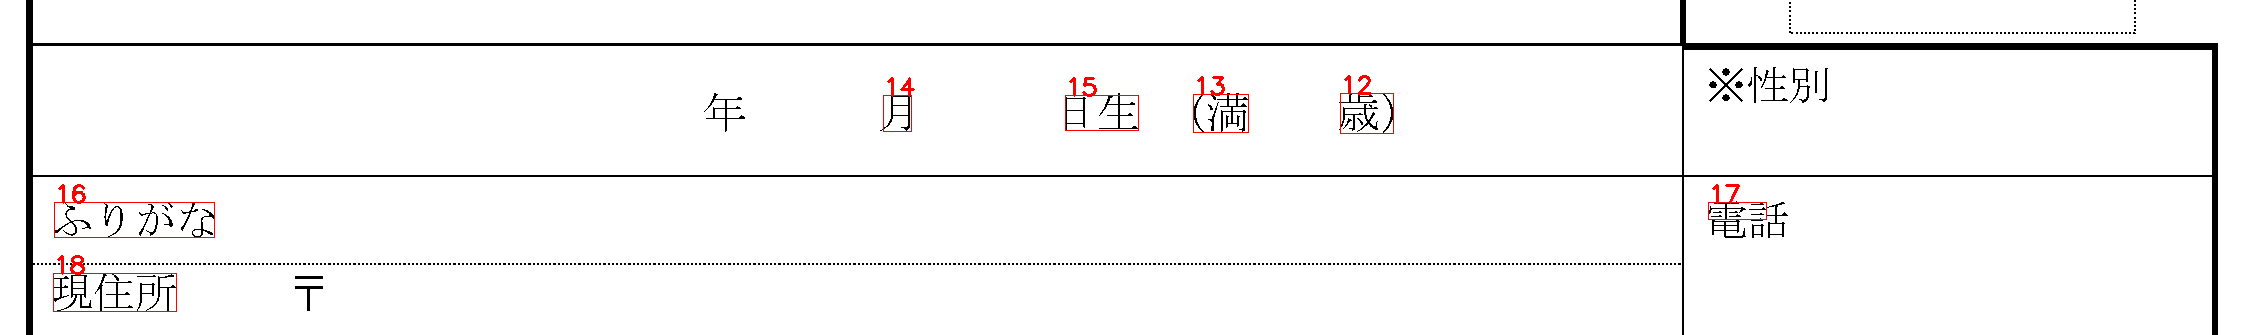
\includegraphics[width=15cm]{image/04-implementation/before_sorted_string.png}
        }
        \caption{誤って番号を割り振った文字位置}
        \label{fig:before_sorted_string}
    \end{center}
\end{figure}
\begin{figure}[tp]
    \begin{center}
        \fbox{
            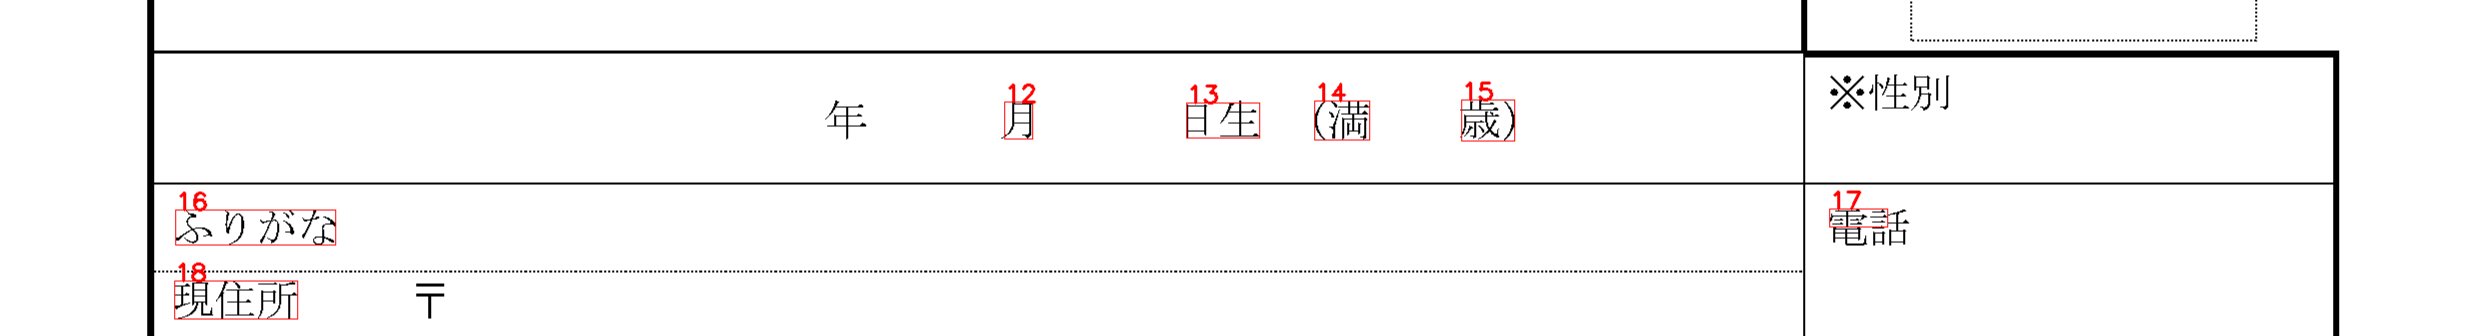
\includegraphics[width=15cm]{image/04-implementation/after_sorted_string.png}
        }
        \caption{再ソートによって昇順に並び替えた文字位置}
        \label{fig:after_sorted_string}
    \end{center}
\end{figure}
ソート後は、図\ref{fig:before_sorted_string}では不具合が発生していた箇所が、図\ref{fig:after_sorted_string}では、左から12番、13番、14番、15番となっており、昇順となっていることがわかる。

図\ref{fig:original}に示した帳票画像に対する、文字情報取得処理の出力をまとめたものを、図\ref{fig:char_recognition_for_original}に示す。
\lstset{language=}
\begin{figure}[tp]
    \begin{lstlisting}
    string[0] ((1644, 244), (1730, 285)) : 番号
    string[1] ((1597, 321), (1724, 363)) : 請求日
    string[2] ((1343, 486), (1411, 528)) : 詩
    string[3] ((1046, 518), (1106, 555)) : 月
    string[4] ((1194, 487), (1260, 555)) : 求
    string[5] ((1354, 530), (1400, 555)) : 較
    string[6] ((898, 683), (983, 725)) : 御中
    string[7] ((223, 992), (926, 1034)) : 下記の通り、ご請求申し上げます。
    string[8] ((1573, 1073), (1662, 1106)) : FAX
    string[9] ((229, 1147), (449, 1189)) : ご請求金額
    string[10] ((1126, 1147), (1248, 1190)) : (税込)
    string[11] ((1574, 1146), (1656, 1187)) : 担当
    string[12] ((1183, 1313), (1270, 1354)) : 数量
    string[13] ((1526, 1311), (1606, 1352)) : 単価
    string[14] ((1970, 1311), (2058, 1352)) : 合計
    string[15] ((1521, 2267), (1608, 2308)) : 小計
    string[16] ((1499, 2343), (1632, 2386)) : 消費税
    string[17] ((1520, 2422), (1608, 2463)) : 合計
    string[18] ((1160, 2576), (1293, 2619)) : 備考
    \end{lstlisting}
    \caption{図\ref{fig:original}から取得した文字}
    \label{fig:char_recognition_for_original}
\end{figure}
また、図\ref{fig:char_recognition_for_original}で表す形式を、図\ref{fig:format_char}に示す。
% \begin{center}
%     string[A]: ((B, C), (D, E)) : (F)
% \end{center}

% \begin{center}
%     \begin{tabular}{l}
%     A: ソート後の番号\\  
%     B: バウンディングボックスの左上頂点のx座標\\
%     C: バウンディングボックスの左上頂点のy座標\\  
%     D: バウンディングボックスの右下頂点のx座標\\
%     E: バウンディングボックスの右下頂点のy座標\\
%     F: 取得文字\\
%     \end{tabular}
% \end{center}
\begin{figure}[tp]
    \begin{center}
        string[A]: ((B, C), (D, E)) : (F)
    \end{center}

    \begin{center}
        \begin{tabular}{l}
        A: ソート後の番号\\  
        B: バウンディングボックスの左上頂点のx座標\\
        C: バウンディングボックスの左上頂点のy座標\\  
        D: バウンディングボックスの右下頂点のx座標\\
        E: バウンディングボックスの右下頂点のy座標\\
        F: 取得文字\\
        \end{tabular}
    \end{center}
    \caption{図\ref{fig:char_recognition_for_original}で取得文字を表示する形式}
    \label{fig:format_char}
\end{figure}
図\ref{fig:char_recognition_for_original}で示す文字位置を参照し、バウンディングボックスを描画した画像を、図\ref{fig:bbox_recognition_for_original}に示す。
\begin{figure}[tp]
    \begin{center}
        \fbox{
            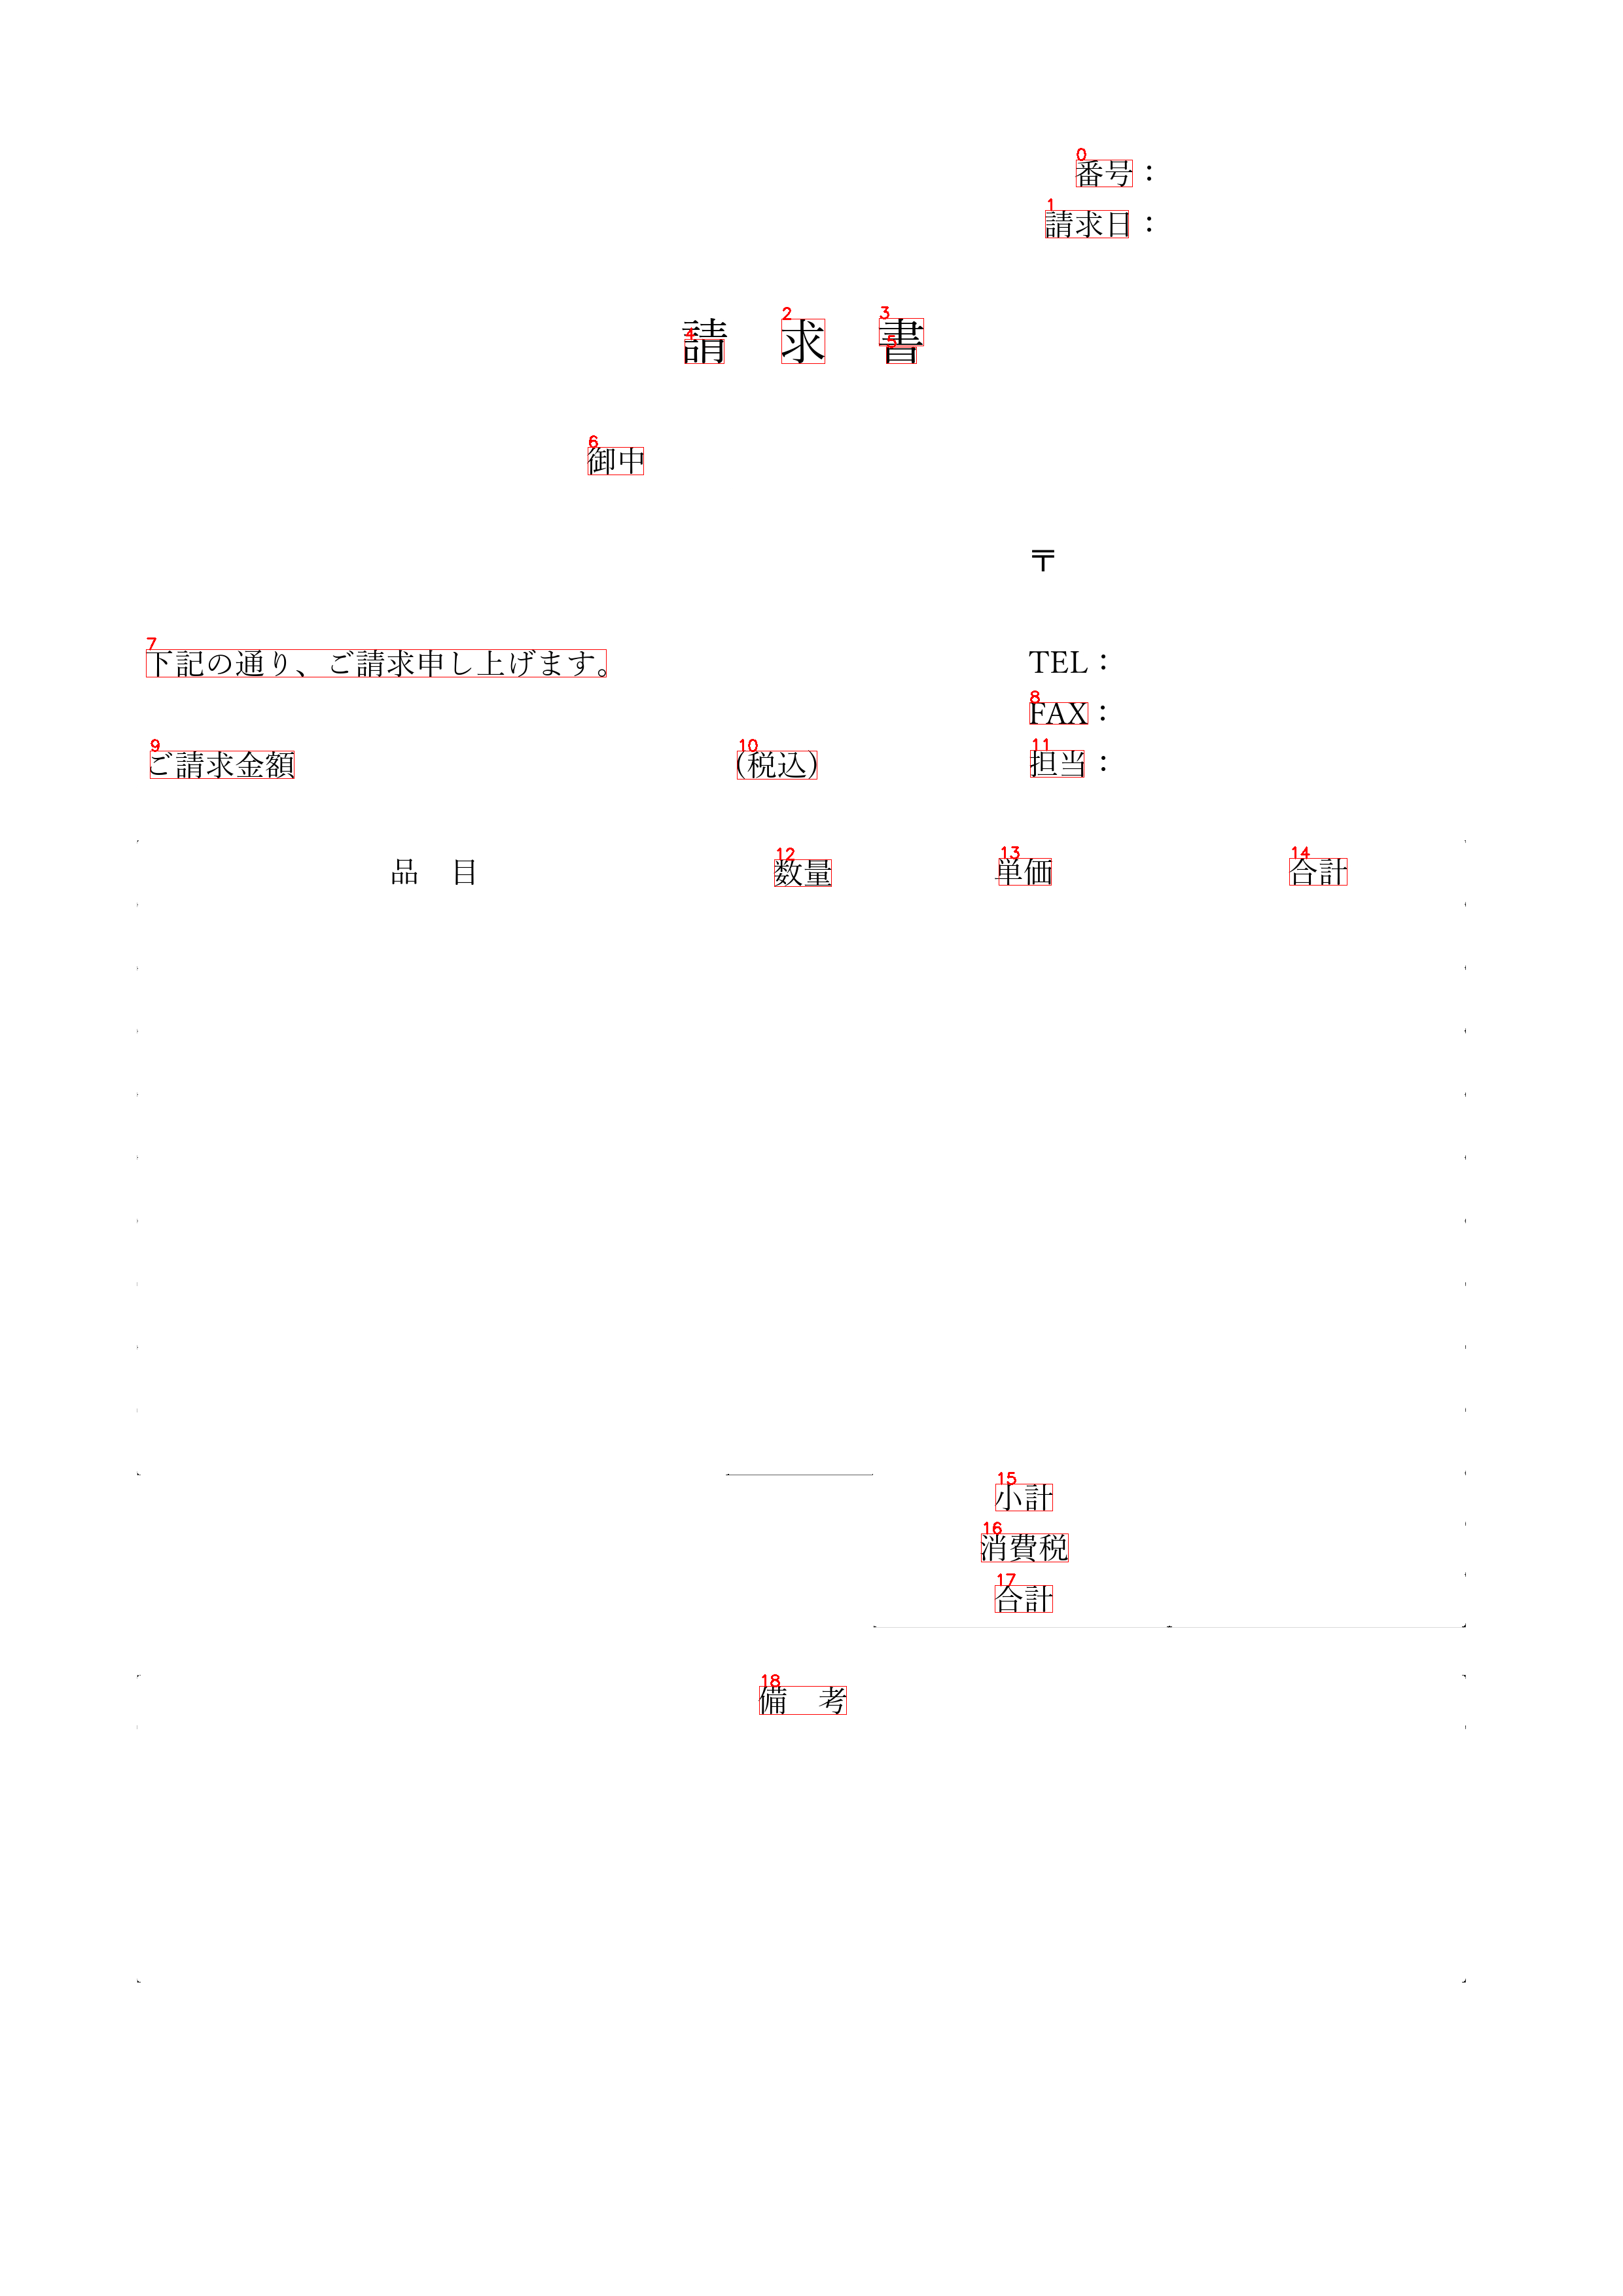
\includegraphics[width=15cm]{image/04-implementation/char_with_bbox.png}
        }
        \caption{図\ref{fig:char_recognition_for_original}の文字位置を図\ref{fig:original}の画像に描画した画像}
        \label{fig:bbox_recognition_for_original}
    \end{center}
\end{figure}
例えば、番号1の取得文字は、「請求日」であり、バウンディングボックスの左上頂点のxy座標が(1597, 321)、バウンディングボックスの右下頂点のxy座標が(1724, 363)となっている。
図\ref{fig:char_recognition_for_original}中の番号は、図\ref{fig:bbox_recognition_for_original}のバウンディングボックスの左上に表示する番号と一致する。

バウンディングボックスを描画していない文字については、認識できなかった文字である。
認識に失敗した文字が及ぼす影響については、\ref{sec:problems}節で後述する。

\subsection{除外判定処理}\label{subsec:exclusion_judgement_processing}
除外判定処理は、属性推測処理(\ref{subsec:att_prediction_processing}節で後述)に不要な文字情報を除外し、出力する処理である。
文字情報取得処理(\ref{subsec:char_information_obtainment_processing}節を参照)の文字情報を入力とし、除外判定処理後の文字情報を出力する。
出力は、属性推測処理(\ref{subsec:att_prediction_processing}節で後述)とラベル割付処理(\ref{subsec:label_link_processing}節で後述)に渡す。

形態素解析ソフトウェアであるFugashiを用いて、取得文字を形態素に分割し、品詞を解析する。
取得文字を構成する形態素の数のうち、特定の品詞である形態素の数の割合が半分以上である場合は、属性推測処理において意味がない取得文字であるとして、該当の文字情報を除外する。
文字を認識する際に、紙面と背景の境界や、領域取得部(\ref{sec:area_coords_obtainment_part}節を参照)で取得できなかった矩形や直線を、文字として誤認識する場合がある。
不要な文字の属性推測処理を防ぐことにより、処理時間を短縮することができる。

以下に、UniDic品詞体系(左からカンマ区切りで、大分類、中分類、小分類、細分類)に基づき、除外対象である形態素の品詞を示す。
分類が``*"となっている場合は、該当する分類がないことを示す。
なお、除外対象とする品詞は、経験から決定している。

\begin{itemize}
    \item 補助記号,一般,*,*
    \item 感動詞,一般,*,*
    \item 感動詞,フィラー,*,*
\end{itemize}

ある帳票画像に対して、\ref{subsec:char_information_obtainment_processing}節で取得したバウンディングボックスを描画した画像の一部を、図\ref{fig:before_exclusion_bbox}に示す。
また、図\ref{fig:before_exclusion_bbox}で描画したバウンディングボックスに対応する取得文字を出力した画像を、図\ref{fig:before_exclusion_string}に示す。
\begin{figure}[tp]
    \begin{center}
        \fbox{
            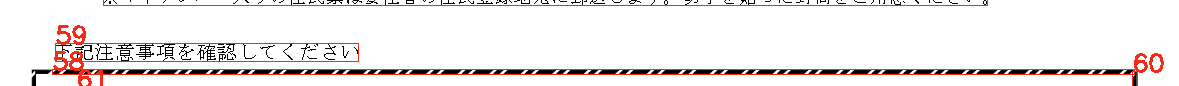
\includegraphics[width=15cm]{image/04-implementation/before_exclusion_bbox.png}
        }
        \caption{属性推測処理に不要な文字を含む文字認識}
        \label{fig:before_exclusion_bbox}
    \end{center}
\end{figure}
図\ref{fig:before_exclusion_bbox}と図\ref{fig:before_exclusion_string}の58番および60番の取得文字は、帳票画像内の矩形の辺を誤って文字として認識している。
この矩形については、矩形領域座標取得処理(\ref{subsec:rect_coords_obtainment_processing}節を参照)で取得できなかったため、背景色の矩形を描画できていない。
図\ref{fig:before_exclusion_bbox}と図\ref{fig:before_exclusion_string}の58番および60番の取得文字は、属性推測処理において意味がない文字である。
図\ref{fig:before_exclusion_string}に示した取得文字に対して除外判定処理を実行し、属性推測処理に不要な取得文字を除外した出力を、図\ref{fig:after_exclusion_string}に示す。
\begin{figure}[tp]
    \begin{center}
        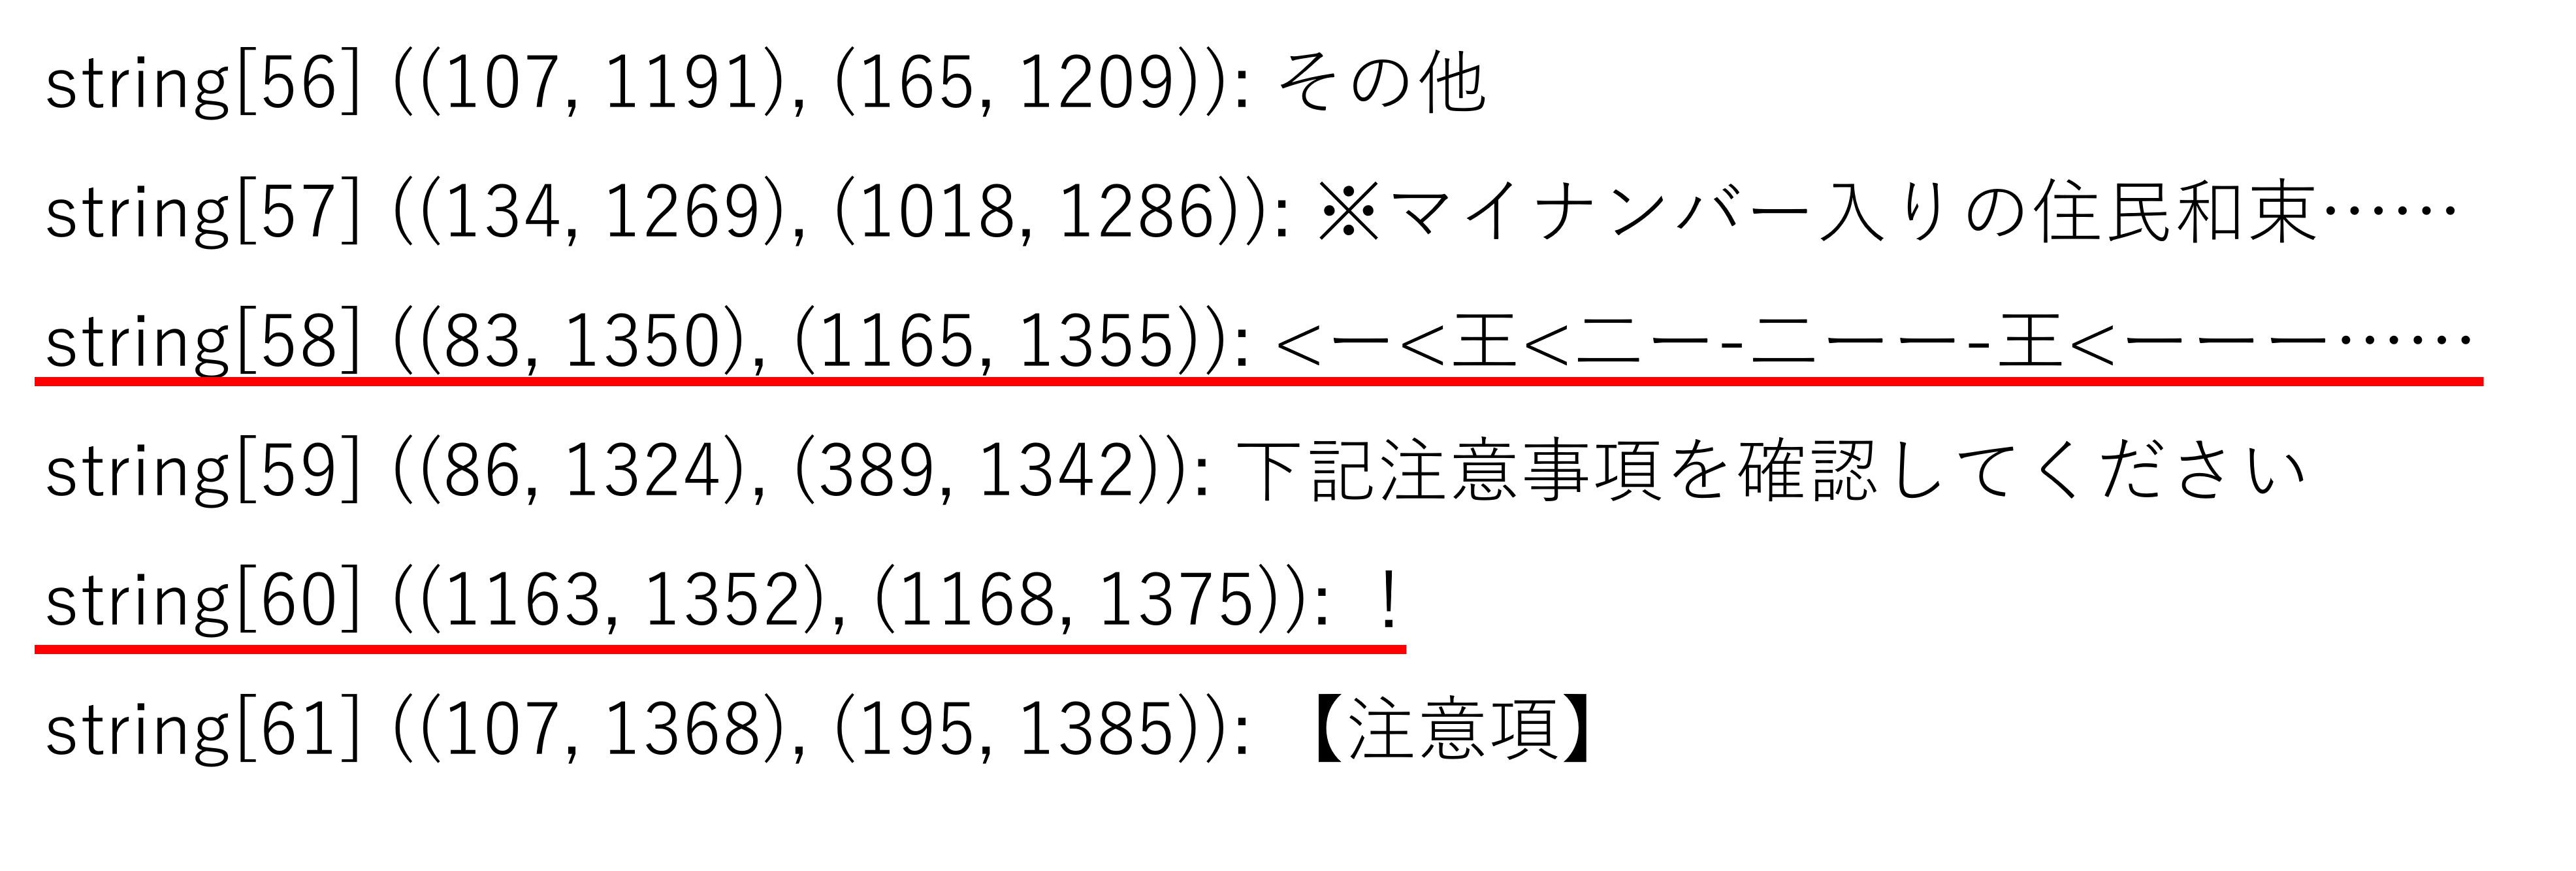
\includegraphics[width=15cm]{image/04-implementation/before_exclusion_string.png}
        \caption{除外判定処理実行前の図\ref{fig:before_exclusion_bbox}の取得文字}
        \label{fig:before_exclusion_string}
    \end{center}
\end{figure}
\begin{figure}[tp]
    \begin{center}
        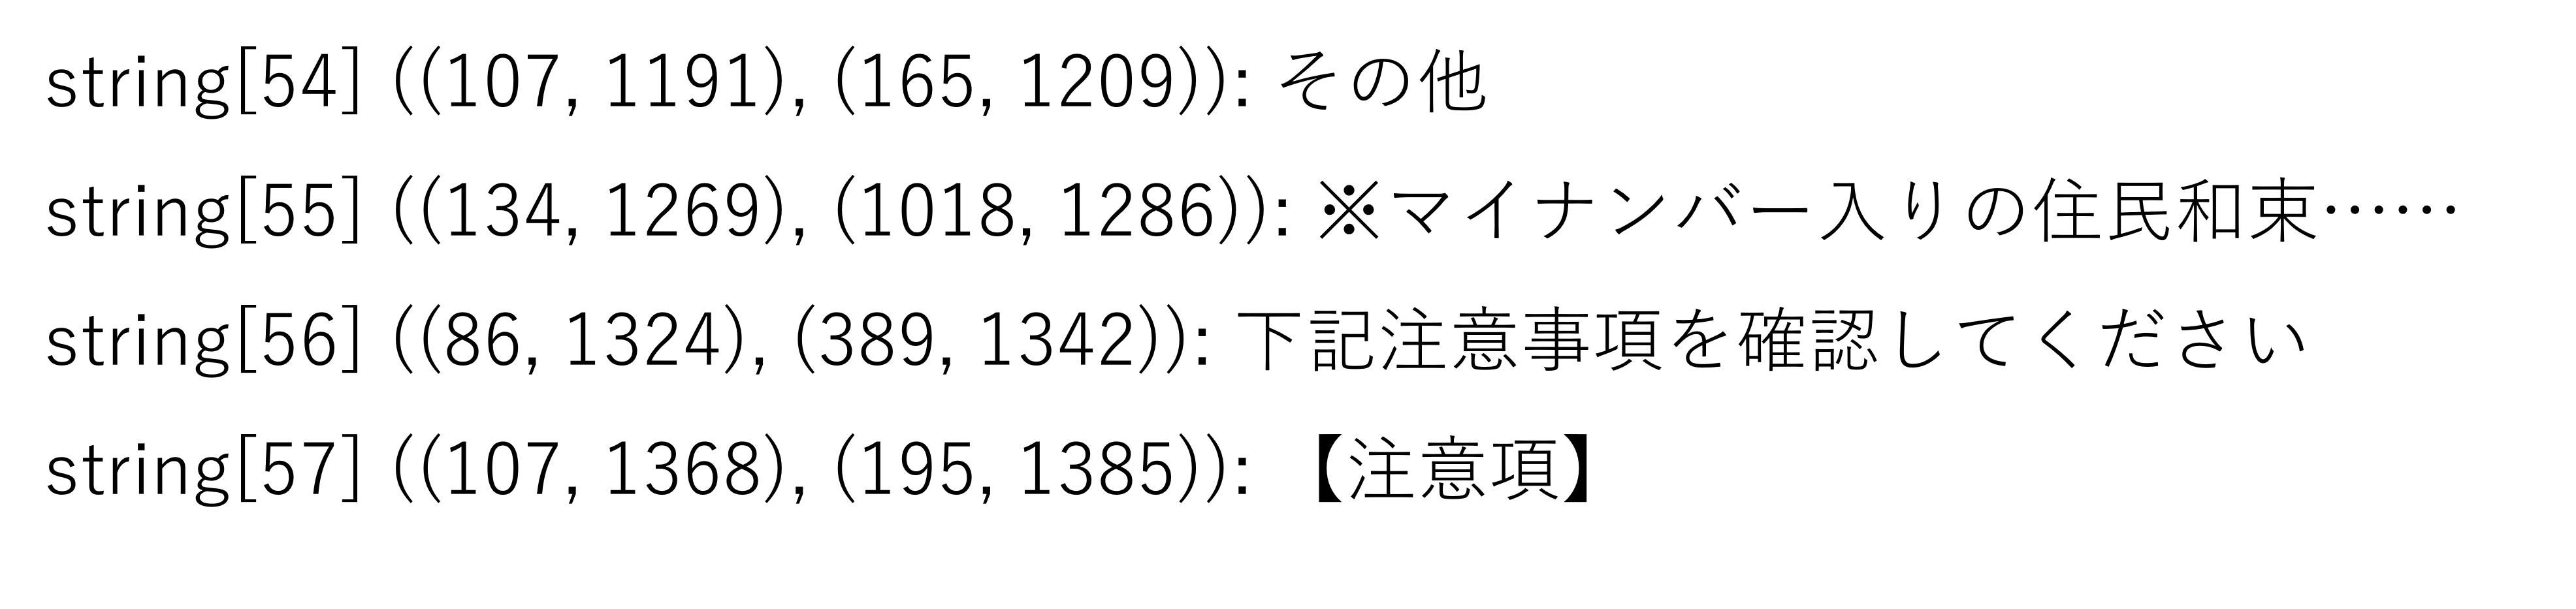
\includegraphics[width=15cm]{image/04-implementation/after_exclusion_string.png}
        \caption{図\ref{fig:before_exclusion_string}の取得文字に対して除外判定処理後の取得文字}
        \label{fig:after_exclusion_string}
    \end{center}
\end{figure}
図\ref{fig:after_exclusion_string}より、除外判定処理によって、属性推測処理に不要な取得文字の除外できたことがわかる。

\section{ラベル割付部}\label{sec:label_link_part}
ラベル割付部では、取得した領域座標に対してラベルを割り付ける処理部である。
領域座標取得部(\ref{sec:area_coords_obtainment_part}節を参照)の領域座標と、除外判定処理(\ref{subsec:exclusion_judgement_processing}節を参照)後の文字情報を入力とし、領域座標とそのラベルを出力とする。
出力は、ファイル出力部(\ref{subsec:file_output_part}節で後述)に渡す。

なお、割り付けるラベルの種類は、領域近傍の取得文字から推測する属性に依存する。

\subsection{属性推測処理}\label{subsec:att_prediction_processing}
属性推測処理では、取得文字に対して、属性である、日付(date)、文字列(string)、数値(number)の中から推測する処理である。
除外判定処理(\ref{subsec:exclusion_judgement_processing}節を参照)後の文字情報を入力とし、取得文字に対応する属性と文字位置を出力とする。
出力は、ラベル割付処理(\ref{subsec:label_link_processing}節で後述)に渡す。

取得文字に対して、属性を、日付(date)、文字列(string)、数値(number)の中から1つ推測する。
属性の推測には、大規模言語モデルYouri(\ref{sec:Youri}節を参照)を用いる。
使用する大規模言語モデルをYouriに選定した理由を、以下に示す。

\begin{itemize}
    \item ローカル環境で推論が可能である\\
        属性推測処理では、帳票画像の文字をプロンプトとして入力する。
        APIを介してプロンプトを外部に送信する場合、帳票画像内に記載された内容が流出する可能性がある。
        帳票には、機密情報や個人情報を含む可能性があるため、ローカル環境で処理を完結する。
    \item 日本語の推論に特化している\\
        Youriは、rinna社が公開した、Llama2に対して日本語の学習データで継続事前学習を行った、大規模言語モデルである。
        日本語の推論に特化しており、推測する属性の精度が高い。
    \item 軽量であり、高速に属性を推測できる\\
        YouriはAPIを介さない他の言語モデルと比較して、高速である。
        属性推測処理では、取得した文字の回数だけYouriにプロンプトを入力し、返答を待つ必要がある。
        属性の推測にかかる時間が短いモデルを選定することで、属性の推測にかかる時間を短縮する。
\end{itemize}

大規模言語モデルは、指示と異なる出力をする場合がある。
そのため、示した3つの属性以外を出力する場合がある。
日付(date)、文字列(string)、数値(number)以外の属性の推測を防ぐため、Youriの出力から3つの属性のいずれかとなるよう補正を行う。
日本語の推論に特化した言語モデルを利用することによって、取得した日本語の文字に対して、属性をより正確に推測できる。

属性推測処理の流れを、以下に示す。
以下の処理は、文字情報取得処理(\ref{subsec:char_information_obtainment_processing}節を参照)でソートを行った順番で、除外判定処理後の取得文字の数だけ繰り返す。
また、Youriに入力するプロンプトの構文を、図\ref{fig:prompt_struct_for_attribute_prediction}に示す。
なお、図\ref{fig:prompt_struct_for_attribute_prediction}における(取得文字)は、除外判定後の取得文字を指す。

\begin{enumerate}
    \item 除外判定処理(\ref{subsec:exclusion_judgement_processing}節を参照)の出力である除外判定後の取得文字を受け取る。
    \item 図\ref{fig:prompt_struct_for_attribute_prediction}に示すプロンプトをYouriに入力し、属性を推測する。
    \item \label{enum:Youri_output}Youriの出力を受けとる。
    \item 以下の順で、\ref{enum:Youri_output}.で受け取ったYouriの出力に対して処理を行い、属性を補正する。
        \begin{enumerate}
            \item 全文字の属性を文字列(string)とする。
            \item 出力に「日」を含む場合は、日付(date)として判定し、属性を文字列(string)から更新し、属性を補正する。
            \item 出力に「数」を含む場合は、数値(number)として判定し、属性を文字列(string)から更新し、属性を補正する。
            \item 出力に「日」、「数」を含まない場合は、属性を更新せず、文字列(string)のままとする。
        \end{enumerate}
\end{enumerate}

\begin{figure}[tp]
    \setbox0\vbox{
        \vbox{\# 命令書:}
        \vbox{以下の制約条件にあてはまるものを出力せよ。}
        \vbox{\# 制約条件:}
        \vbox{・記入欄に記入する内容が、日付、文字列、数値の中から、どのデータ型が最も適切であるかを選択する。}
        \vbox{・出力は短く、あてはまるデータ型のみとする。}
        \vbox{・例として、年月日などは日付、氏名などは文字列、金額などは数値があてはまる。}
        \vbox{(取得文字)という欄は、どのデータ型に該当するか。}
    }
    \centerline{\fbox{\box0}}
    \caption{取得文字の属性を推測するプロンプトの構文}
    \label{fig:prompt_struct_for_attribute_prediction}
\end{figure}

図\ref{fig:char_recognition_for_original}に示した取得文字に対して、Youriが出力したテキストの一部を、以下の図\ref{fig:output_Youri}に示す。
\lstset{language=}
\begin{figure}[tp]
    \begin{lstlisting}
        数値に該当する。 (番号)
        日付 (請求日)
        詩は、文字列に該当する。 (詩)
        日付 (月)
        日付 (求)
        数値 (較)
        日付 (御中)
        日付 (下記の通り、ご請求申し上げます。)
        数字です。 (FAX)
        数値 (ご請求金額)
        「(税込)」は、数値のデータ型に該当します。 ((税込))
        文字列 (担当)
        数値 (数量)
        数値型に該当する (単価)
        数値 (合計)
        数値 (小計)
        数値 (消費税)
        数値 (合計)
        備考は、文字列に該当する。 (備考)
    \end{lstlisting}
    \caption{図\ref{fig:char_recognition_for_original}に示した取得文字からYouriが出力したテキスト}
    \label{fig:output_Youri}
\end{figure}
図\ref{fig:output_Youri}は、Youriの出力のうち、左にYouriの返答を、右の括弧内に取得文字を示す。
図\ref{fig:output_Youri}の1行目や3行目は、「番号」、「詩」という取得文字に対して、文を出力している。

図\ref{fig:output_Youri}で示したYouriの出力から、属性を補正した結果を、図\ref{fig:predict_att_for_original}に示す。
\lstset{language=}
\begin{figure}[tp]
    \begin{lstlisting}
        att[0]: number (番号)
        att[1]: date (請求日)
        att[2]: string (詩)
        att[3]: date (月)
        att[4]: date (求)
        att[5]: number (較)
        att[6]: date (御中)
        att[7]: date (下記の通り、ご請求申し上げます。)
        att[8]: number (FAX)
        att[9]: number (ご請求金額)
        att[10]: number ((税込))
        att[11]: string (担当)
        att[12]: number (数量)
        att[13]: number (単価)
        att[14]: number (合計)
        att[15]: number (小計)
        att[16]: number (消費税)
        att[17]: number (合計)
        att[18]: string (備考)
    \end{lstlisting}
    \caption{図\ref{fig:output_Youri}のYouriの出力から補正した属性を属性した結果}
    \label{fig:predict_att_for_original}
\end{figure}
また、図\ref{fig:predict_att_for_original}で表す形式を、図\ref{fig:format_att}に示す。
\begin{figure}[tp]
    \begin{center}
        att[A]: B (C)
    \end{center}

    \begin{center}
        \begin{tabular}{l}
            A: ソート後のインデックス\\
            B: 属性を推測した結果\\
            C: 推測対象である取得文字\\
        \end{tabular}
    \end{center}
    \caption{図\ref{fig:predict_att_for_original}で属性を表示する形式}
    \label{fig:format_att}
\end{figure}
例えば、1番の取得文字は、「請求日」であり、推測した属性は日付(date)となる。4番の取得文字は、「月」であり、推測した属性は文字列(string)となる。
図\ref{fig:predict_att_for_original}の番号は、図\ref{fig:bbox_recognition_for_original}のバウンディングボックスの左上頂点に表示する番号、および図\ref{fig:char_recognition_for_original}で示した番号と一致する。
なお、大規模言語モデルによる出力に依存して属性を決定するため、常に正しい属性を推測することはできていない。
例えば、6番の取得文字である「御中」の属性を、日付(date)と推測している。
御中は組織や団体の敬称であり、本来は文字列(string)の属性が正しい。

\subsection{ラベル割付処理}\label{subsec:label_link_processing}
ラベル割付処理では、取得した領域座標に対して、近傍に存在する文字の属性を割り付ける。
領域座標取得部(\ref{sec:area_coords_obtainment_part}節を参照)の領域座標、属性推測処理(\ref{subsec:att_prediction_processing}節を参照)の属性と文字列を入力とし、領域座標とそのラベルを出力する。
出力は、JSONファイル出力処理(\ref{subsec:json_file_output_processing}節で後述)と領域強調画像出力処理(\ref{subsec:area_highlighted_image_output_processing}節で後述)に渡す。

ラベル割付処理の流れを、以下に示す。
以下の処理は、文字位置取得処理でソートを行った順番で、除外判定処理(\ref{subsec:exclusion_judgement_processing}節を参照)後の取得文字の数だけ繰り返す。

\begin{enumerate}
    \item \label{enum:bbox_center} バウンディングボックスの拡張点のxy座標を参照し、中心点のxy座標を計算する。
    \item 取得した領域座標のうち、矩形領域は右下頂点のxy座標、下線部領域は右端点のxy座標と、計算した中心点のxy座標を比較する。
    \item \ref{enum:bbox_center}.で計算した中心点のx座標とy座標が共に大きい全ての領域座標をラベル割付の対象として、文字位置に対応する取得文字の属性をラベルとして割り付ける。
    \item 繰り返し処理によって、既にラベルを割り付けた領域座標がラベル割付の対象となった場合は、後の処理で割り付けるラベルに更新する。
          これによって、日本語の帳票を書き進める順番に対応して、別の領域座標のラベルを割り付けることを防ぐ。
\end{enumerate}

以上の繰り返し処理を行った後、領域座標に対して、ラベルを割り付ける。

\section{ファイル出力部}\label{subsec:file_output_part}
ファイル出力部は、領域座標と、領域座標に対応するラベルを組とするJSON形式のファイル、および、JSONファイルの取得領域を強調表示したPNG形式の画像2枚を出力する処理部である。
ラベル割付処理(\ref{subsec:label_link_processing}節を参照)の領域座標とそのラベルを入力とし、JSONファイルと2枚の領域強調画像を出力とする。

\subsection{JSONファイル出力処理}\label{subsec:json_file_output_processing}
JSONファイル出力処理は、取得した領域座標とラベルを整形し、領域座標と、領域座標に対応するラベルを組とするJSONファイルを出力する処理である。
ラベル割付処理(\ref{subsec:label_link_processing}節を参照)の領域座標とそのラベルを入力とし、それらをまとめたJSONファイルを出力とする。

出力するJSONファイルは、配列rects\_dataと配列underlines\_dataで構成し、矩形領域の情報、下線部領域の情報をそれぞれ持つ。
これら2つの配列は、それぞれ以下の情報をもつ。

\begin{itemize}
    \item 配列ごとに一意であるid
    \item 領域に割り付けているラベルを示すlabel
    \item 領域座標を示すオブジェクトcoords
\end{itemize}

配列rects\_dataと、配列underlines\_dataを、図\ref{fig:example_output_json}に示す形式に整形後、JSONファイルを出力する。

\subsection{領域強調画像出力処理}\label{subsec:area_highlighted_image_output_processing}
領域強調画像出力処理は、取得した領域座標より、帳票画像に対して領域を描画することで、取得した領域座標を強調表示した2枚の画像を出力する処理である。
領域座標取得部(\ref{sec:area_coords_obtainment_part}節を参照)で取得した領域座標と、ラベル割付処理(\ref{subsec:label_link_processing}節を参照)で取得したラベルを入力とし、矩形と直線を、割り付けたラベルと共に描画した2枚の画像を出力とする。

出力する画像については、矩形領域強調画像と、下線部領域強調画像の計2枚の画像を出力する。
矩形領域強調画像については、矩形をランダムなRGBカラーで描画することで、矩形領域を強調表示する。
さらに、左上頂点に、JSONファイル内のrects\_data配列のidキーの値と、labelキーの値を表示する。
下線部の帳票画像内記入欄については、緑色で下線部領域の直線を描画することによって、下線部領域を強調表示する。
さらに、左端点の上に、JSONファイル内のunderlines\_data配列のidキーの値と、labelキーの値を表示する。
これにより、人間が目視でJSONファイルを確認する場合と比較して、取得した領域座標と割り付けたラベルの確認が容易となる。

以下に、矩形と直線を、割り付けたラベルと共に描画した画像を出力する流れを示す。

\begin{enumerate}
    \item ラベル割付処理(\ref{subsec:label_link_processing}節を参照)から、領域座標と、領域座標に対応するラベルを、それぞれ取得する。
    \item Pythonのcopy関数により、入力である帳票画像をコピーし、2枚の帳票画像A、Bを生成する。
    \item \label{enum:randint}Numpy(\ref{sec:Numpy}節を参照)のrandint関数を用いて、3つのランダムな整数値を生成し、それぞれを各色空間の値とすることで、ランダムなRGBカラーを決定する。
    \item 帳票画像Aに対して、OpenCVのdrawContours関数と\ref{enum:randint}.で生成したRGBカラーを用いて、矩形領域座標を参照して矩形を描画する。
    \item 帳票画像Bに対して、OpenCVのline関数を用いて、下線部領域座標を参照して直線を描画する。
    \item OpenCVのputText関数(\ref{sec:OpenCV}節を参照)を用いて、idキーの値と、labelキーの値を、各領域座標の左上に描画する。
    \item OpenCVのimwrite関数を用いて、帳票画像Aと帳票画像Bを、それぞれ矩形領域強調画像と下線部領域強調画像として保存する。
\end{enumerate}

以上の処理後、矩形領域強調画像と、下線部領域強調画像を出力する。
ある帳票画像に対して、試作したツールを適用し、出力した矩形領域強調画像と、下線部領域強調画像を、それぞれ図\ref{fig:img_rect_labels}と図\ref{fig:img_underline_labels}に示す。
\begin{figure}[tp]
    \begin{center}
        \fbox{
            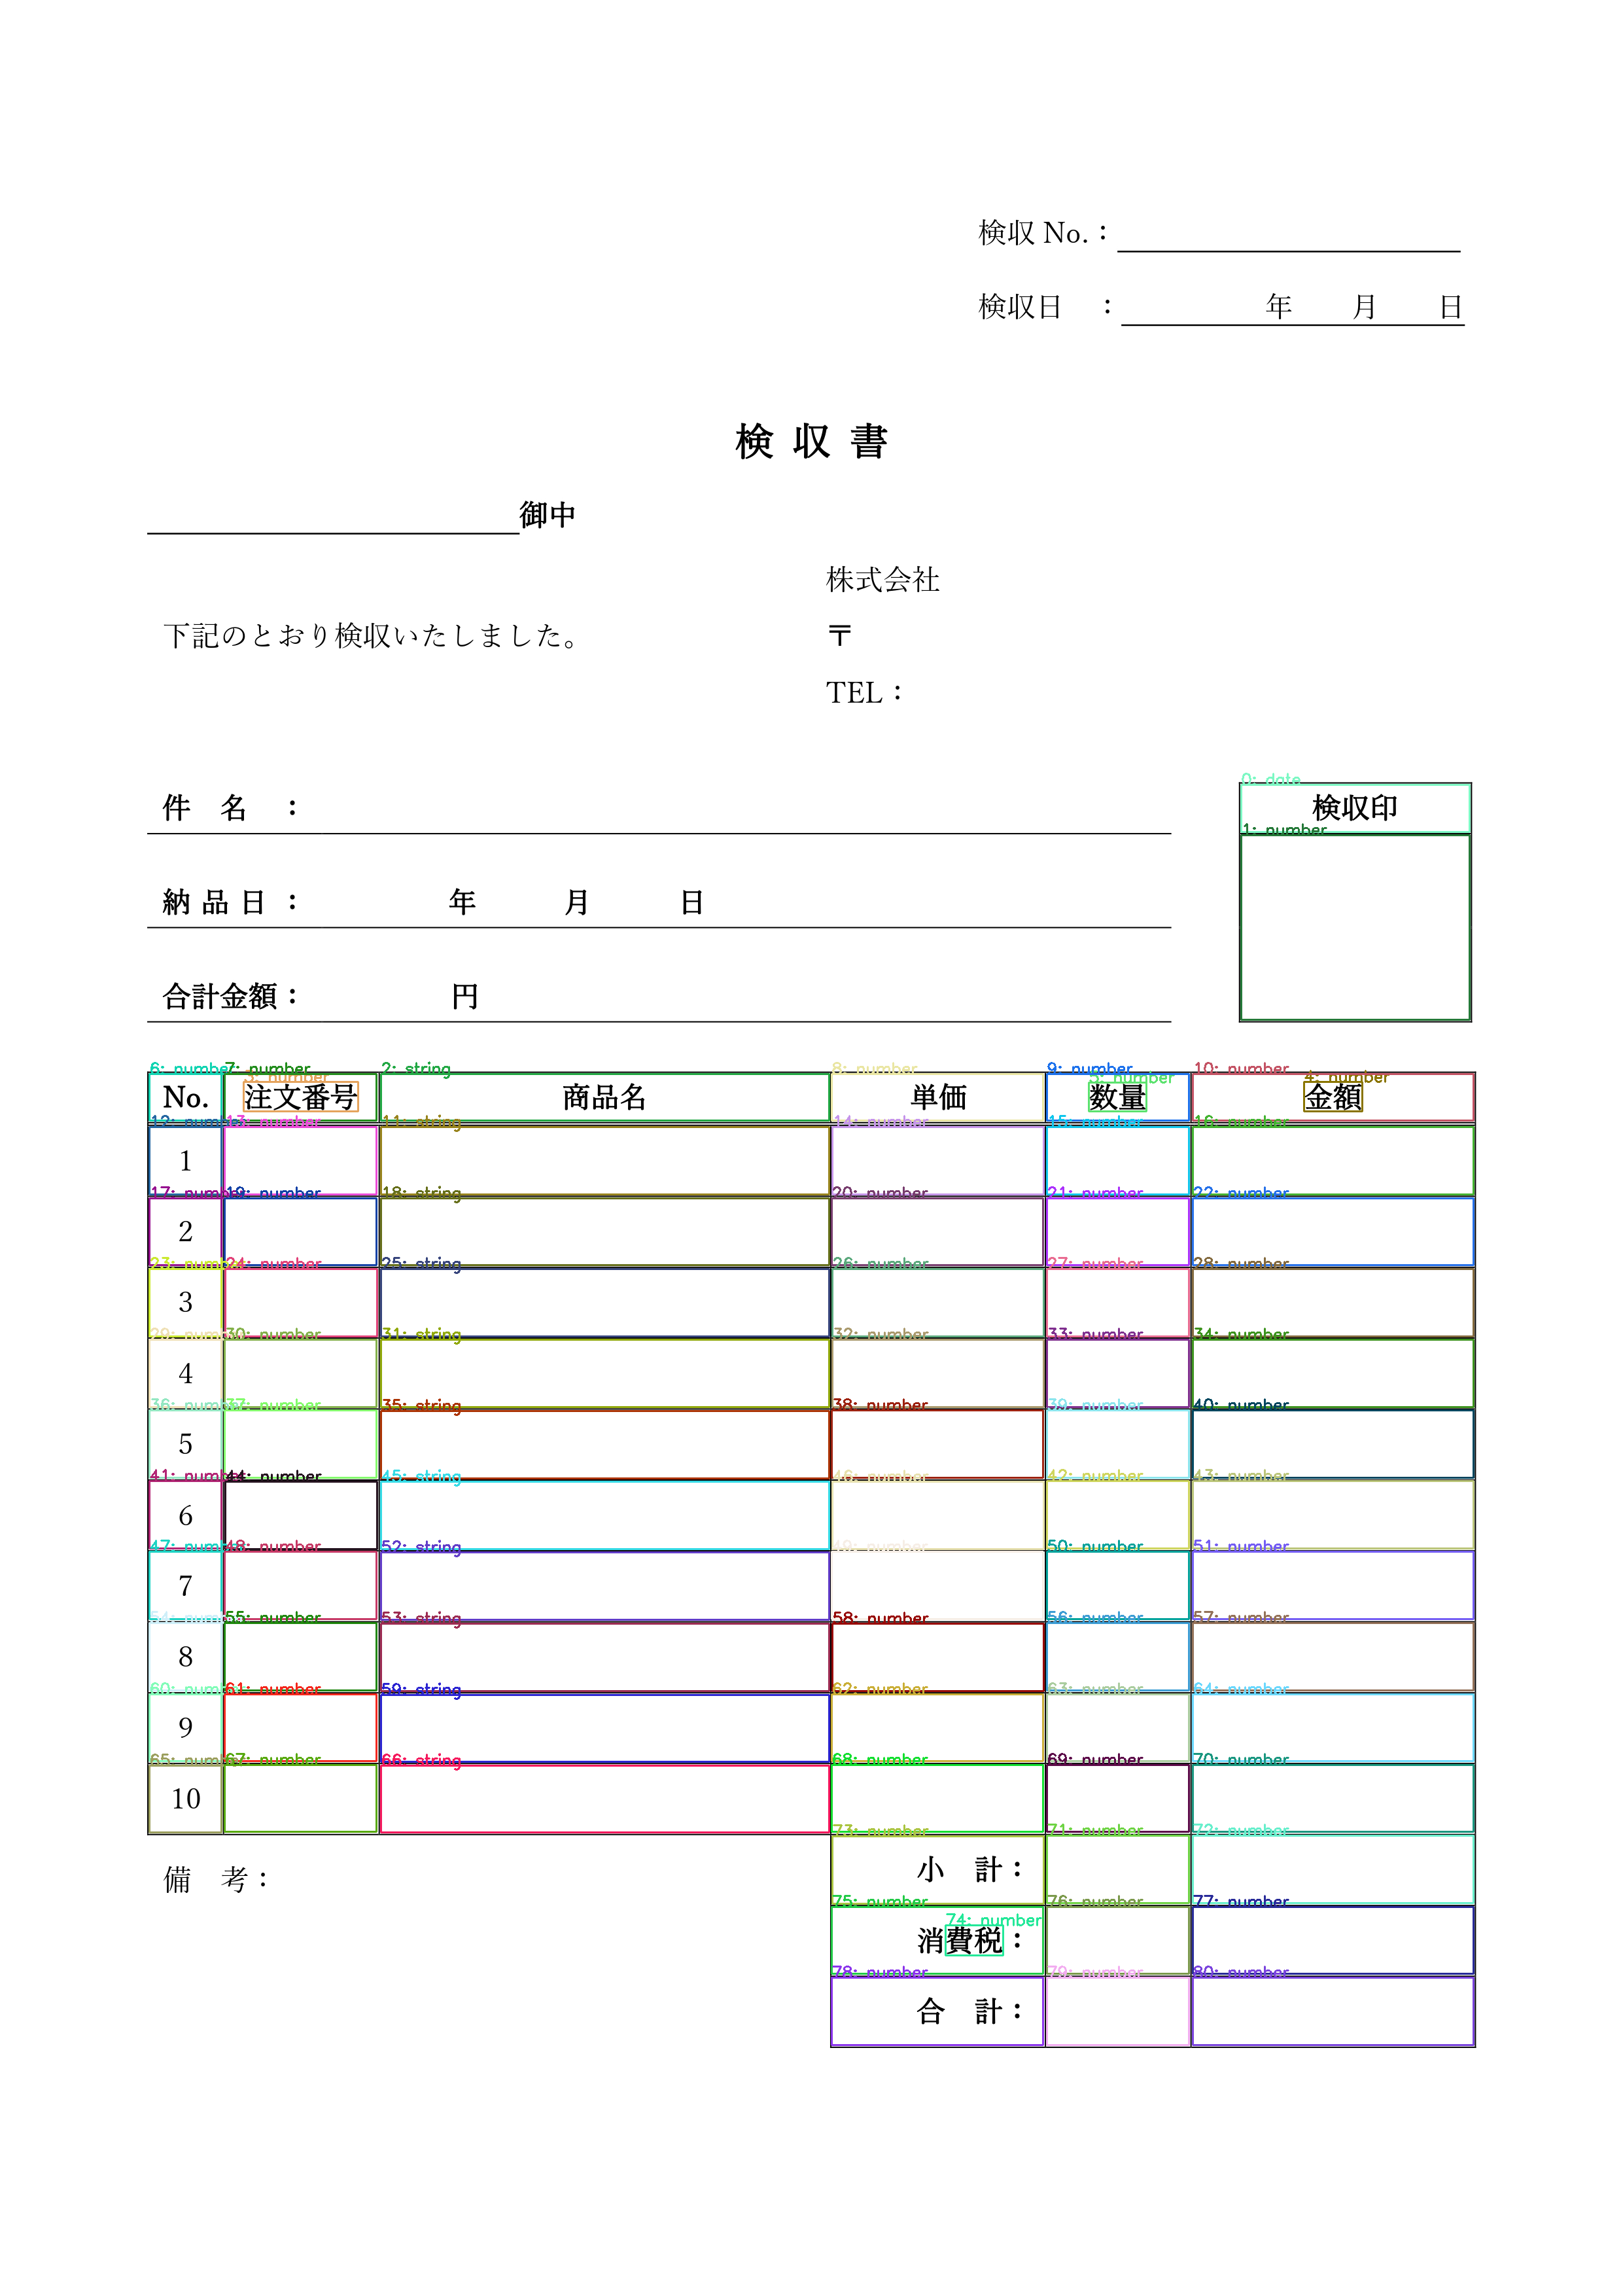
\includegraphics[width=15cm]{image/04-implementation/img_rect_labels.png}
        }
        \caption{ある帳票画像に対して出力した矩形領域強調画像}
        \label{fig:img_rect_labels}
    \end{center}
\end{figure}
\begin{figure}[tp]
    \begin{center}
        \fbox{
            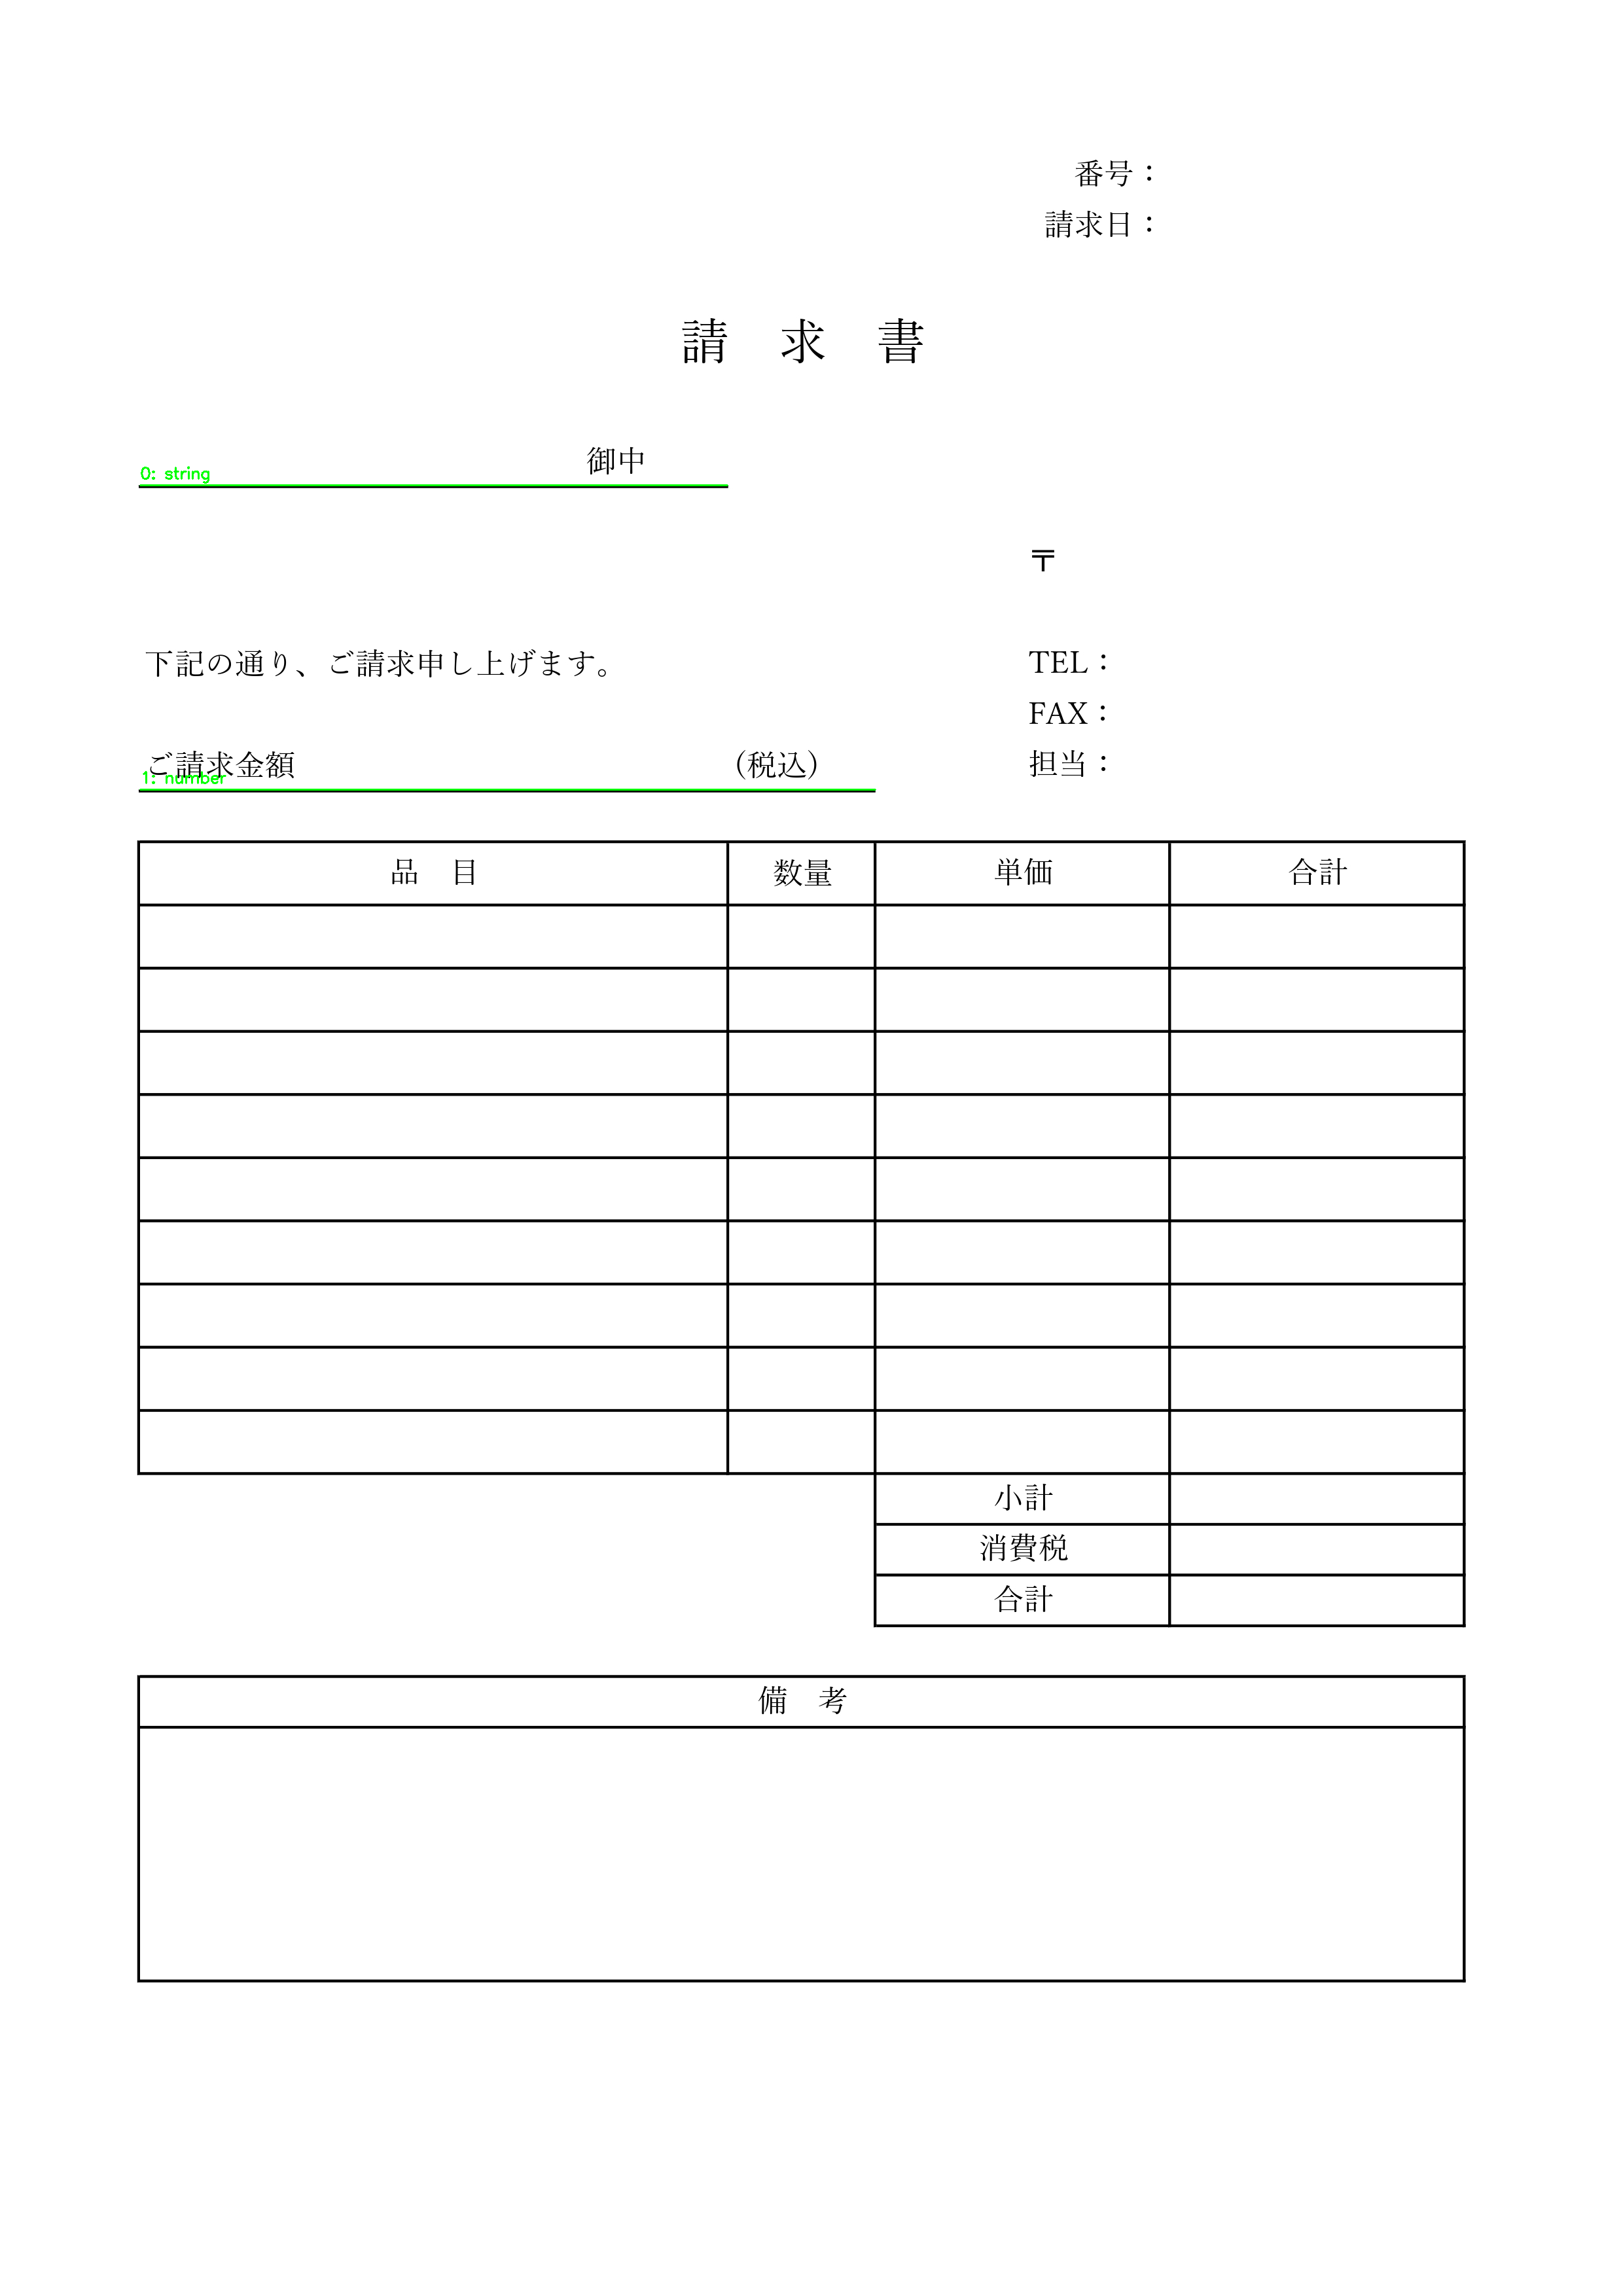
\includegraphics[width=15cm]{image/04-implementation/img_underline_labels.png}
        }
        \caption{ある帳票画像に対して出力した下線部領域強調画像}
        \label{fig:img_underline_labels}
    \end{center}
\end{figure}